\documentclass{article}

\usepackage[italian]{babel}
\usepackage[a4paper,top=2cm,bottom=2cm,left=2.5cm,right=2.5cm,marginparwidth=1cm]{geometry}

% Useful packages
\usepackage{tabularx}
\usepackage{graphicx}
\usepackage[colorlinks=true, allcolors=blue]{hyperref}
\usepackage[inkscapelatex=false]{svg}
\usepackage[table]{colortbl}

\title{Med Portal \\
        Applicativo di supporto nei servizi di emergenza sanitaria
        \\ \large Elaborato per l'esame di Ingegneria del Software}

\author{Matteo Simonetti}
\date{}
\hypersetup{linkcolor=black}
\begin{document}
    \maketitle
    \tableofcontents

    \newpage

    \section{Statement iniziale}

    Si vuole realizzare un applicativo telematico che faciliti la comunicazione tra la squadra sul campo e la centrale in remoto. Tale sistema deve gestire lo scambio di informazioni tra centrale, squadra e triage, permettere il monitoraggio della missione durante il servizio sanitario, e fornire funzionalità di base per gestire schede di missione, login-logout dei mezzi e della squadra, credenziali dei soccorritori registrati, e visualizzare lo storico degli interventi per fini di fatturazione.

    \subsection{Ruolo della centrale}
    Il cittadino in difficoltà chiama il NUE\footnote{Numero Unico di Emergenza} 112 oppure il 118 e dichiara di aver bisogno di assistenza sanitaria comunicando al centralino la propria posizione. Qualora si utilizzi l’applicazione mobile “Where Are U” la centrale riceve automaticamente il nome e la posizione geo-localizzata del paziente. Successivamente comunica l’accaduto e lo stato di salute del paziente.
    Il tecnico della centrale esegue una prima valutazione e in base allo scenario decide di attivare sul luogo uno o più mezzi di soccorso, che possono essere un’ambulanza BLS-D\footnote{Basic Life Support Defibrillation}, ambulanza con infermiere oppure auto-medica. Per fare ciò l’operatore inizia una nuova scheda-missione che viene compilata con la prima valutazione, luogo di obiettivo e un riferimento (solitamente è il nome del chiamante). Viene deciso anche il codice di attivazione (verde, giallo o rosso) e se i mezzi inviati sono autorizzati ad usare i dispositivi acustici.
    A questo punto la scheda viene inviata alle squadre attivate.
    La data e l’ora della chiamata e dell’inizio della missione (quando la squadra riceve la scheda) vengono automaticamente registrati sulla scheda.
    La centrale può osservare in tempo reale la posizione dei mezzi grazie al loro transponder integrato.
    La squadra, formata da al più 4 soccorritori (3 se il mezzo è l’auto-medica), riceve sul tablet il dispatch della missione con codice di attivazione, posizione e la prima valutazione che ha redatto l’infermiere al telefono.

    \subsection{Ruolo dell’autista}
    A questo punto l’autista della squadra invia lo stato di partenza dalla sede inserendo il chilometraggio del mezzo utilizzato. Facoltativamente, può poi scegliere di usufruire del navigatore.
    L’autista ha sempre l’obbligo di aggiornare il proprio stato quando arriva sull’obiettivo, rientra in pronto soccorso (con l’opportuno codice concordato con la centrale), finisce la missione e rientra in sede. Ogni stato che viene inviato viene registrato sulla scheda con allegati data e ora.
    Quando l’autista invia lo stato “partenza da obiettivo”, la scheda della missione viene inviata al terminale del triage del pronto soccorso di destinazione, così da essere consultata dall’infermiere di turno.
    Alternativamente il paziente può rifiutare il trasporto. In tal caso, invece di andare in pronto soccorso, la missione finisce e la squadra rientra.
    Quando il mezzo è rientrato in sede, l’autista invia lo stato e firma la scheda inserendo il chilometraggio finale del mezzo. A quel punto la scheda rimane immutabile e a disposizione per essere consultata in seguito.
    Può succedere che la centrale invii una nuova missione alla squadra prima del loro rientro in sede.
    Allora l’autista, invece di inviare lo stato di rientro in sede, clicca su “Passa a prossima missione”. L’applicativo richiede di inserire il chilometraggio del mezzo, fa firmare la scheda e passa automaticamente sulla scheda della nuova missione.

    \subsection{Ruolo della squadra}
    \subsubsection{Login della squadra}
    A inizio turno la squadra smontante effettua il logout, mentre la squadra operativa fa il login.
    Ogni membro della squadra per effettuare il login deve inserire username (il proprio codice fiscale) e la password personale. Il soccorritore dovrà essere regolarmente registrato sul portale dell’associazione. Nel caso di primo login la password sarà del tipo “nomecognome”, e successivamente l’utente verrà rimandato a una schermata dove dovrà decidere la propria password privata.
    Sempre tramite l’applicativo si devono specificare trai soccorritori chi è l’autista e chi è il caposquadra.
    Se non era stato fatto in precedenza, bisogna selezionare il mezzo tra quelli disponibili della propria associazione.

    \subsubsection{L'intervento}
    La squadra di soccorritori ha il compito di valutare la situazione del paziente, acquisendo parametri vitali e dati anagrafici (se disponibili). Tutti i dati devono essere scritti sulla piattaforma e sincronizzati con la centrale. In base ai parametri, la centrale comunica (via cavo/radio) il codice di rientro e il pronto soccorso di destinazione. Alternativamente il tecnico della centrale può decidere se impiegare risorse aggiuntive come un’altra ambulanza, auto-medica o elisoccorso.
    Eventualmente il paziente può rifiutare il trasporto firmando digitalmente un modulo.
    Nel caso in cui il mezzo di soccorso deve fare rendez-vous con un altro mezzo (eg: elisoccorso), l’autista (o la squadra) del primo mezzo deve selezionare sull’applicativo la voce “Rendez-vous con altro mezzo” nel campo “Esito trattamento”. Questa procedura abilita l’invio tramite l’interfaccia grafica dello stato di rendez-vous.
    Durante interventi congiunti, le squadre attivate per la missione possono sincronizzarsi i dati anagrafici del paziente per evitare perdite di tempo. Per fare ciò bisogna seguire la seguente procedura: la squadra che invia i dati inserisce in un campo il numero della squadra ricevente, mentre quest’ultima deve avere la scheda della missione aperta. La squadra ricevente può o meno accettare i dati in arrivo.

    \subsection{Ruolo dell’associazione}
    Anche l’associazione ha delle credenziali che permettono l’uso della piattaforma. I responsabili possono gestire i mezzi disponibili, registrare nuovi soccorritori e consultare le schede di missione per fini di fatturazione.
    Per registrare un nuovo soccorritore bisogna inserire i dati anagrafici e una copia delle certificazioni da lui conseguite (incluse data di conseguimento e di scadenza).
    È possibile che un soccorritore sia iscritto a più associazioni. In tal caso l’inserimento di alcune certificazioni (tipo quelle rilasciate dal 118) non è necessario e verranno recuperate automaticamente dalla base dati.
    Comunque il passaggio della registrazione è obbligatorio. Questo per far sì che sia possibile tracciare le associazioni a cui il soccorritore appartiene (per esempio per fini di assicurazione da infortuni) e per impedire che altre associazioni utilizzino le credenziali di personale non associato.

    \section{Diagrammi e documentazione}
    \subsection{Casi d'uso}
    Dallo statement iniziale si possono evidenziare quali sono gli attori principali che si interfacciano con il sistema, ovvero la centrale 118, la squadra di soccorso (composta da un autista e almeno un soccorritore) e l'associazione di appartenenza della squadra.
    Di seguito vengono riportati i diagrammi dei casi d'uso con i relativi templates (in fondo a questo documento) e dei mockup di interfaccia grafica.

    \begin{figure}[!h]
        \centering
        %\includesvg[width=4in]{diagrams/svg/ControlCenter!UseCaseDiagram_Centrale_0}
        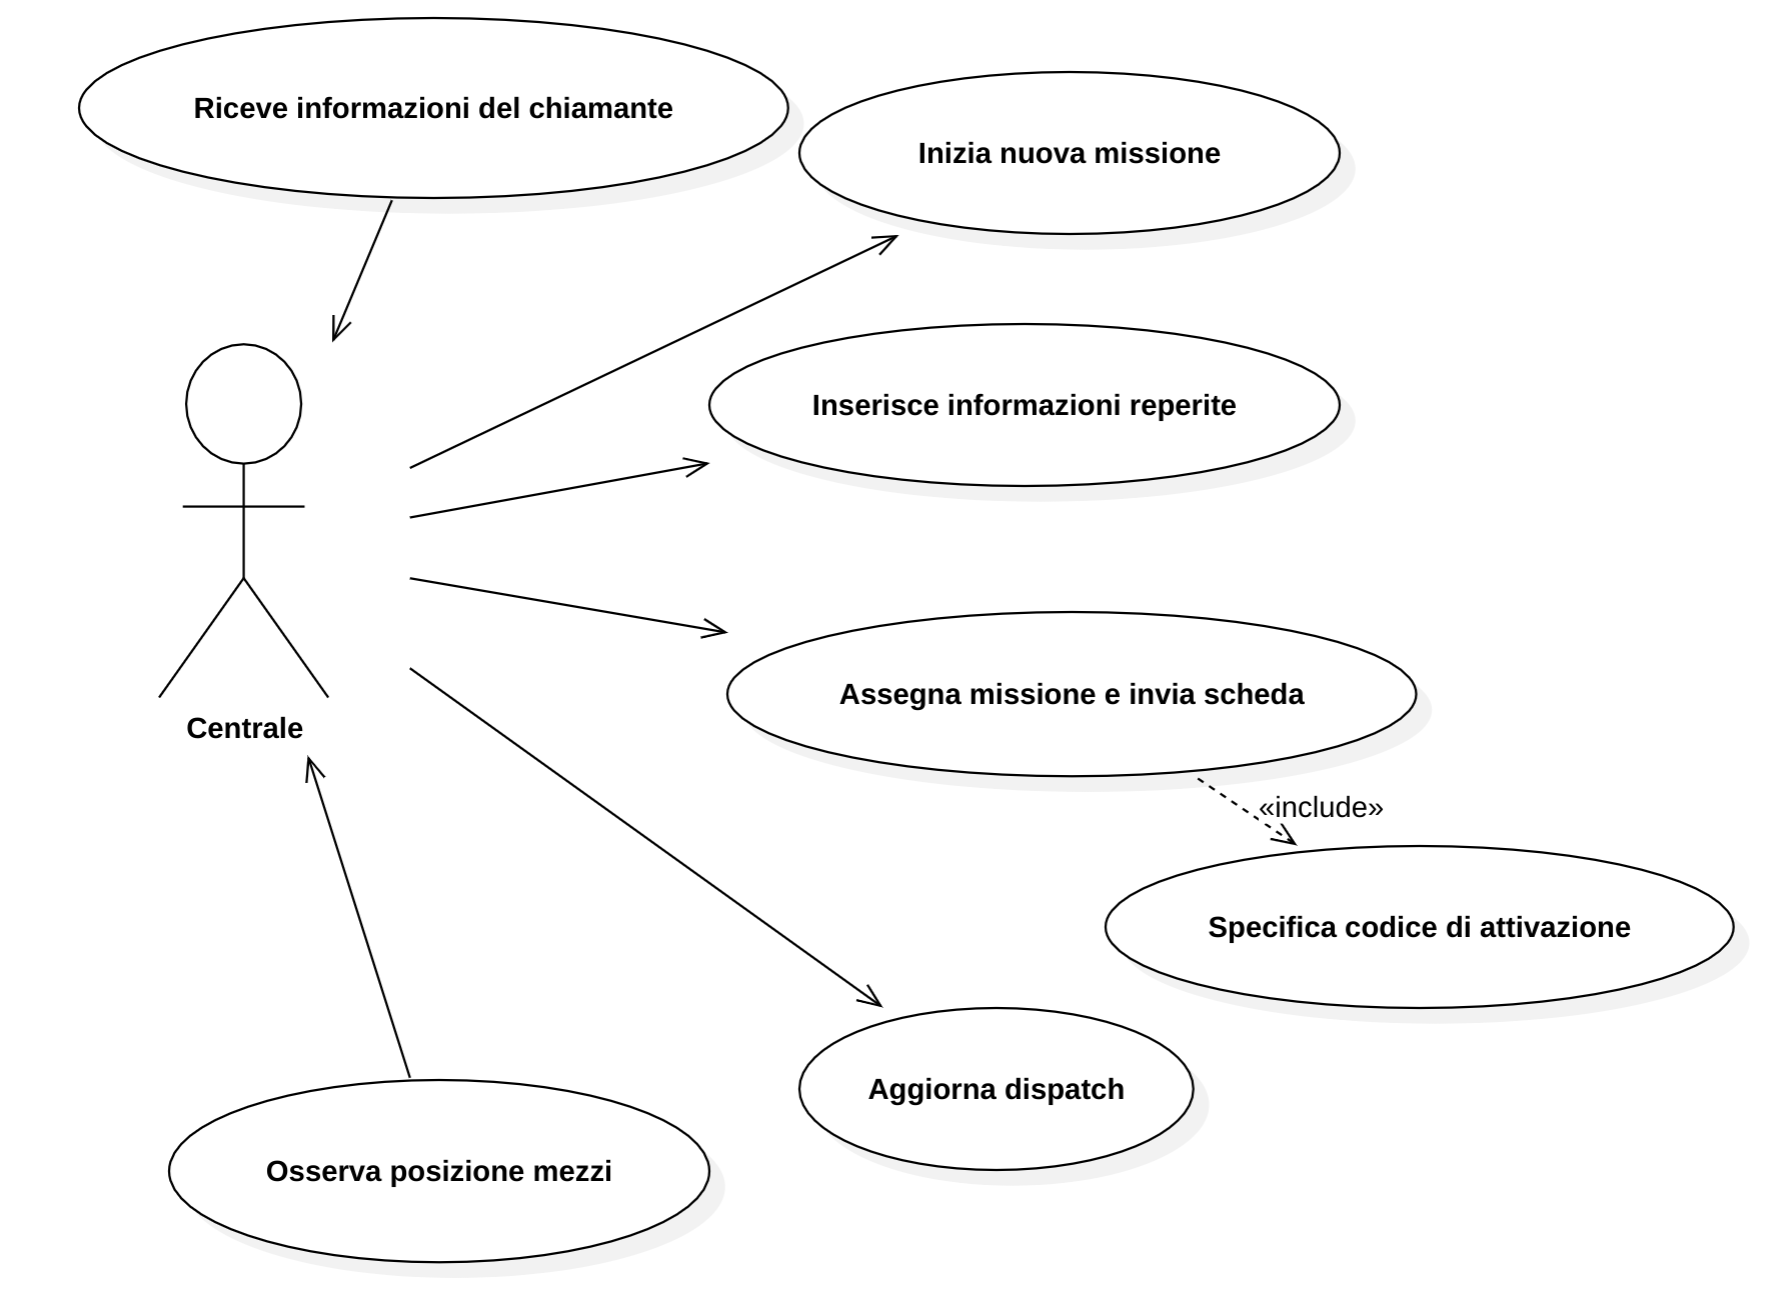
\includegraphics[width=5.5in]{diagrams/png/uc-centrale.png}
        \caption{Diagramma casi d'uso per la centrale}
        \label{fig:uc-controlcenter}
    \end{figure}
    \begin{figure}
        \centering
        %\includesvg[width=5in]{diagrams/svg/Squadra!UseCaseDiagram_Squadra_1}
        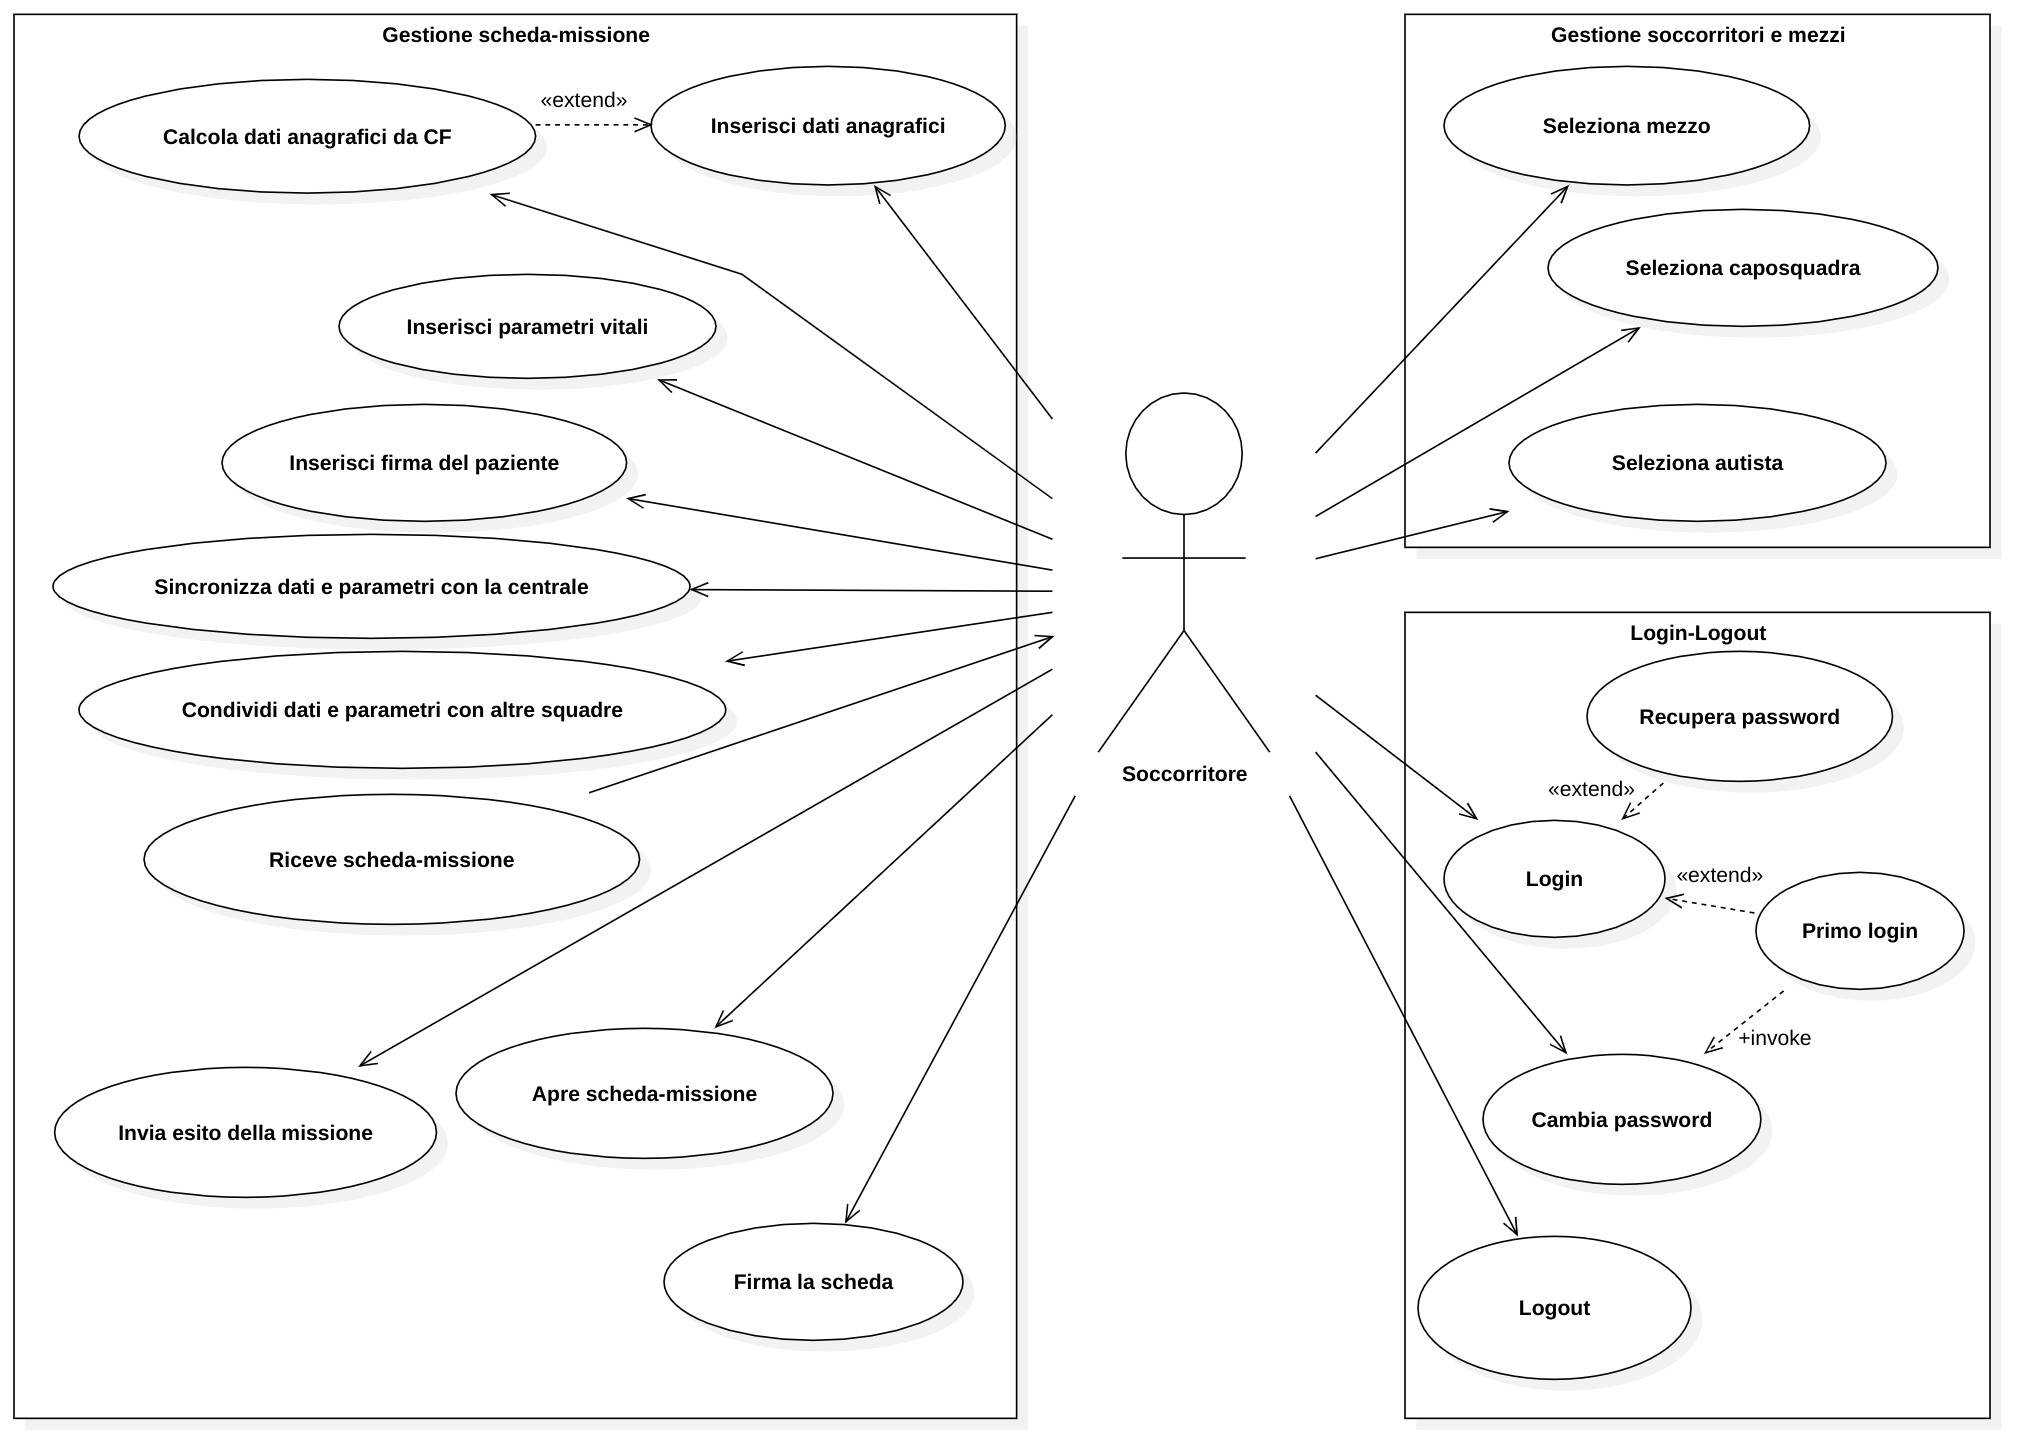
\includegraphics[width=6.5in]{diagrams/png/uc-soccorritore.png}
        \caption{Diagramma casi d'uso per la squadra}
        \label{fig:uc-rescueteam}
    \end{figure}
    \begin{figure}
        \centering
        %\includesvg[width=4in]{diagrams/svg/Autista!UseCaseDiagram_Autista_2}
        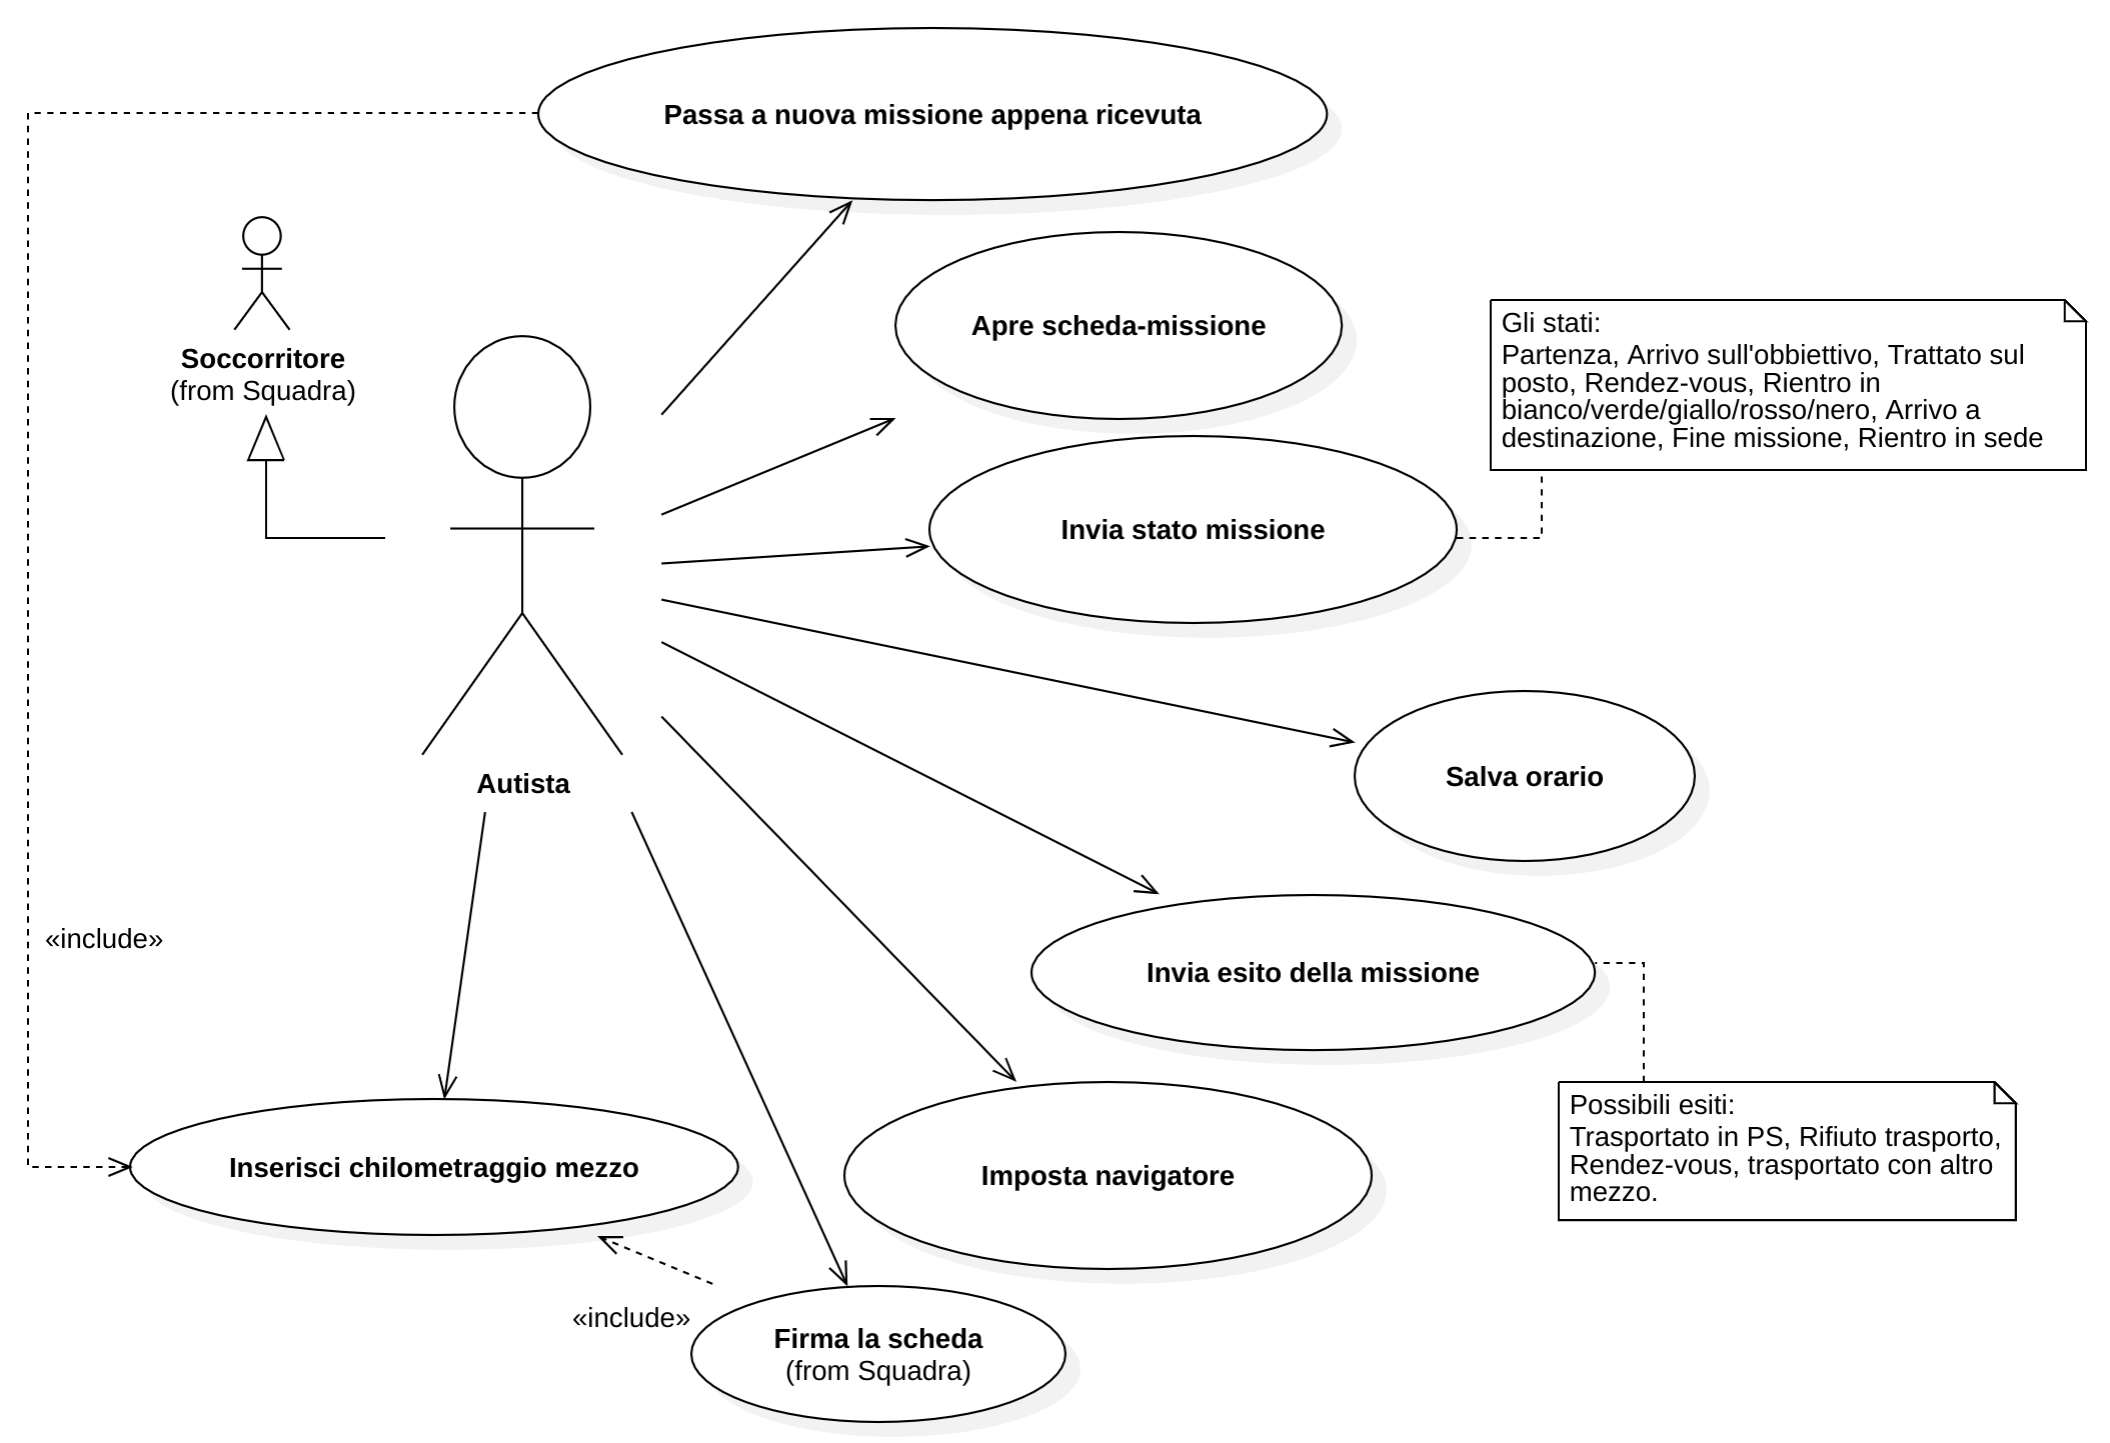
\includegraphics[width=5in]{diagrams/png/uc-autista.png}
        \caption{Diagramma casi d'uso per l'autista}
        \label{fig:uc-autista}
    \end{figure}
    \begin{figure}
        \centering
        %\includesvg[width=3in]{diagrams/svg/Organization!UseCaseDiagram_Associazione_3}
        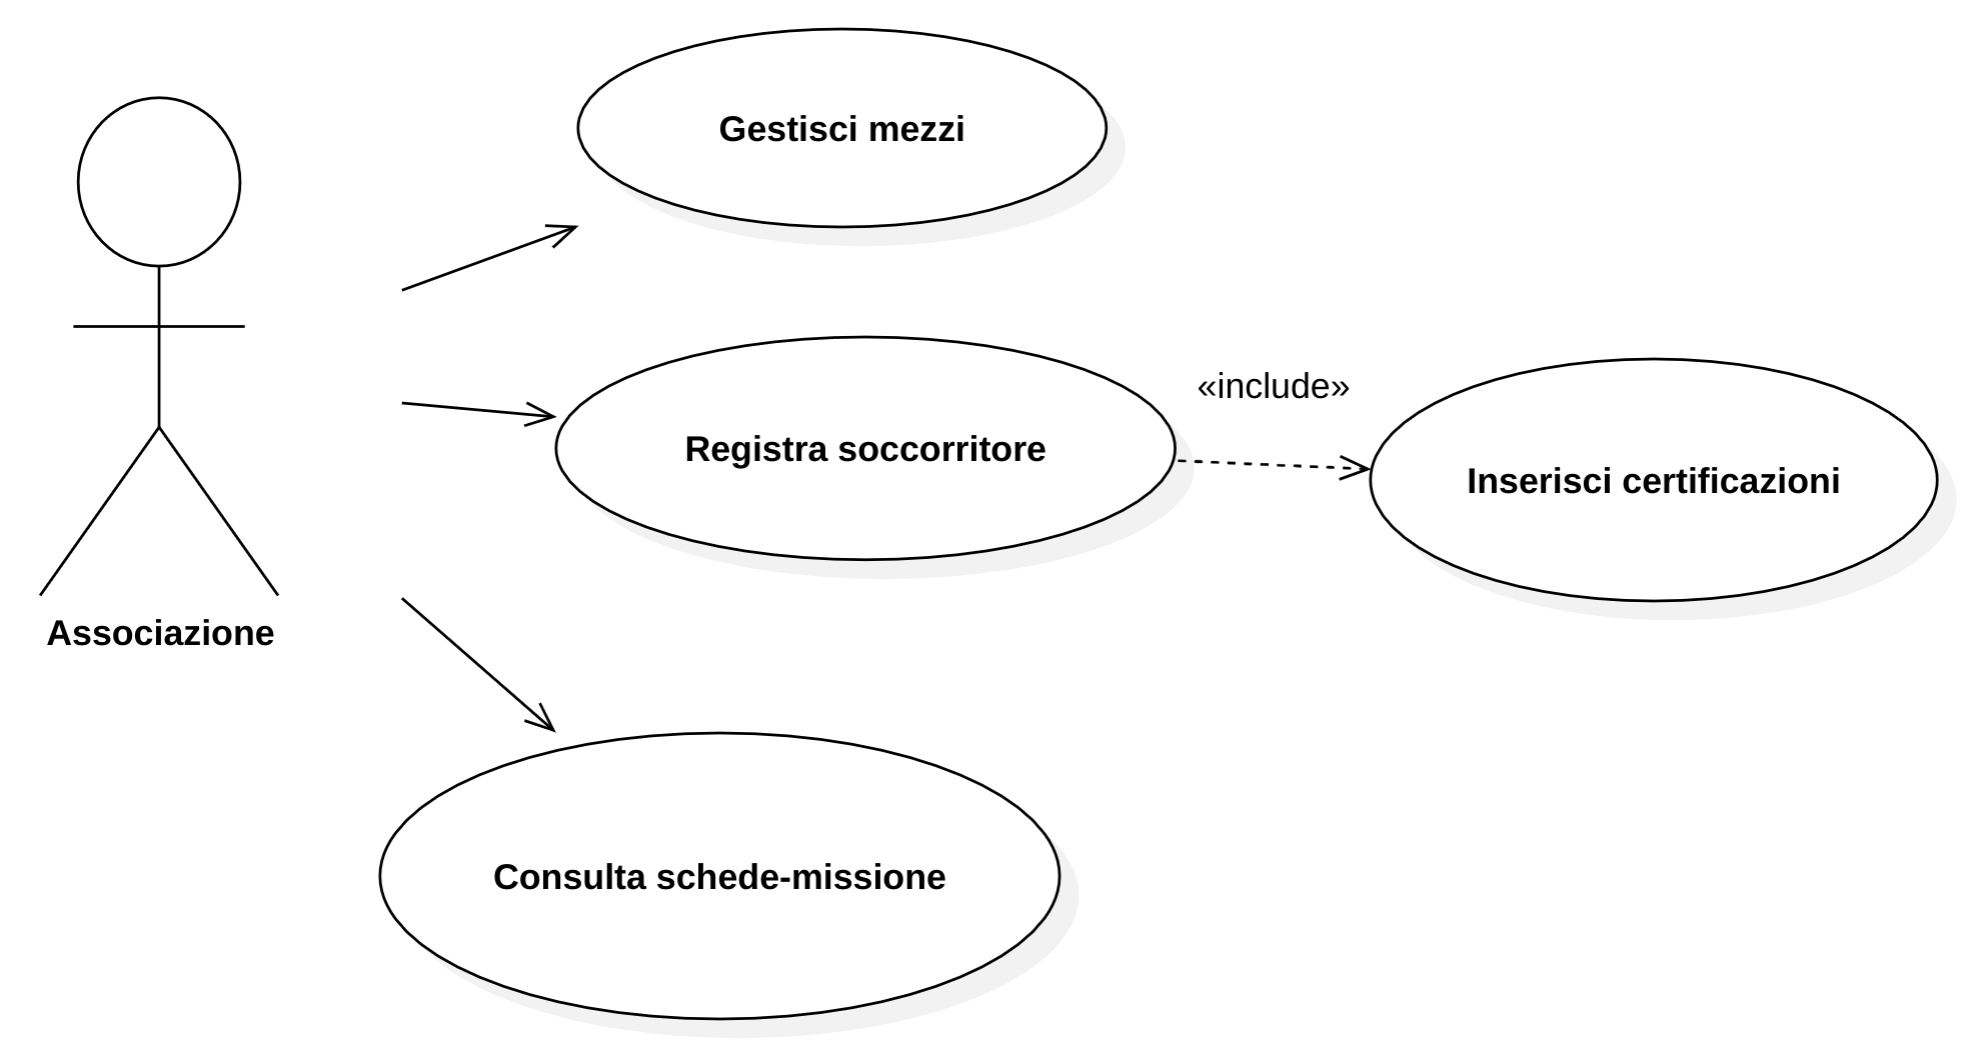
\includegraphics[width=4.5in]{diagrams/png/uc-associazione.png}
        \caption{Diagramma casi d'uso per l'organizzazione}
        \label{fig:uc-organization}
    \end{figure}

    \begin{figure}
        \centering
        \includesvg[width=5.5in]{diagrams/svg/mockup-controlcenter}
        \caption{Interfaccia applicativo della centrale}
        \label{fig:mockup-controlcenter}
    \end{figure}
    \begin{figure}
        \centering
        \includesvg[width=5.5in]{diagrams/svg/mockup-soccorritore}
        \caption{Interfaccia applicativo della squadra}
        \label{fig:mockup-soccorritore}
    \end{figure}
    \begin{figure}
        \centering
        \includesvg[width=3in]{diagrams/svg/mockup-autista}
        \caption{Interfaccia applicativo dell'autista}
        \label{fig:mockup-autista}
    \end{figure}

    \subsection{Architettura e diagramma delle classi}
    Per la realizzazione del progetto è stata scelta l'architettura 3-tier Business logic - Object-relational mapper - Domain model.
    La suddivisione dei packages è avvenuta tenendo conto dell'eventuale transizione da un'applicazione monolitica come è adesso ad una a microservizi.
    In particolare i packages principali sono quelli emersi facendo un'analisi dei $bounded-context$, ovvero $ControlCenter$, $Ems$ e $Organization$.
    Ognuno di questi è suddiviso nei packages $BusinessLogic$, $DataAccess$ e $DomainModel$.
    \newline In $BusinessLogic$ si trovano tutti i $controller$ che implementano ed espongono tutte le funzionalità elencate nei casi d'uso.
    \newline In ogni contesto, il livello $DataAccess$ è composto da sole interfacce. Ciò rende la persistenza dei dati più flessibile al cambio di tipologia di database e il testing più semplice.
    \newline Il $DomainModel$ è composto da tutte le classi e relazioni che caratterizzano il modello di dominio in questione.

    \subsubsection{ControlCenter}
    \begin{figure}
        \centering
        %\includesvg[width=6in]{diagrams/svg/ControlCenter!ControlCenter_0}
        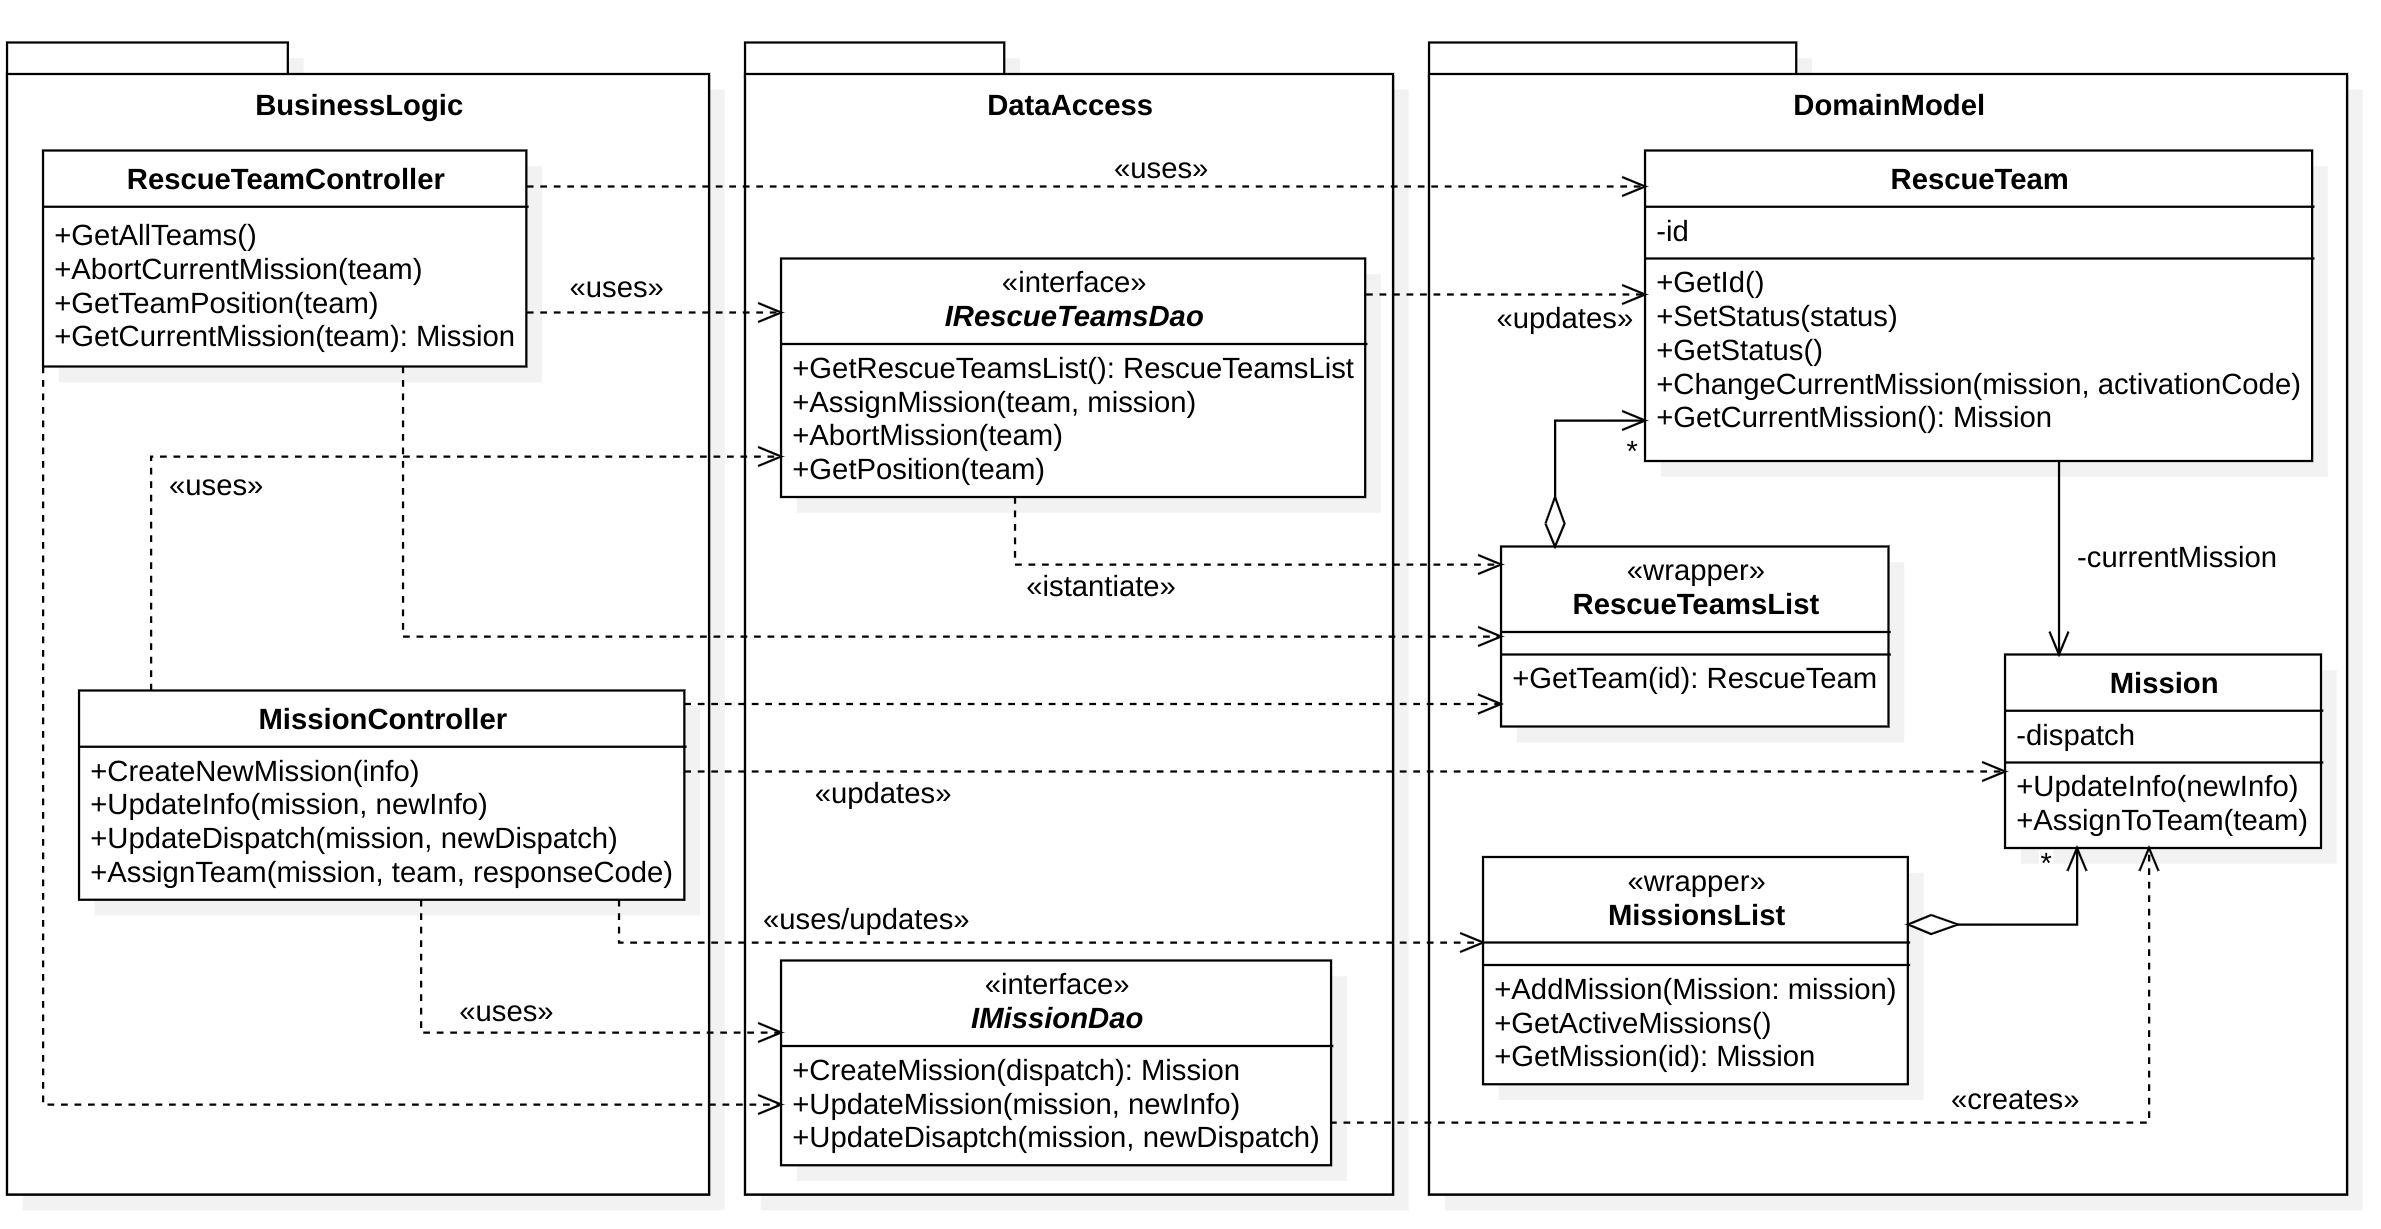
\includegraphics[width=6in]{diagrams/png/uml-controlcenter.png}
        \caption{Diagramma delle classi di ControlCenter}
        \label{fig:uml-controlcenter}
    \end{figure}
    In questo package (figura \ref{fig:uml-controlcenter}) sono presenti $RescueTeamController$ e $MissionController$. La prima classe fornisce metodi di gestione delle squadre di soccorso sul territorio,
    la seconda espone metodi di creazione e gestione delle missioni.
    Entrambi i $controller$, siccome sono responsabili del salvataggio dei dati su database e sincronizzazione del $DomainModel$, dipendono da dei $DataAccessObject$, in questo caso dalle interfacce $IRescueTeamsDao$ e $IMissionDao$.
    Il $DomainModel$ è caratterizzato da una $RescueTeamsList$ e da una $MissionsList$, che tengono traccia rispettivamente delle squadre di soccorso operative e delle missioni di soccorso attualmente in svolgimento.
    Queste due classi non sono altro che dei $Wrapper$ di liste che contengono una collezione di $RescueTeam$ e $Mission$.
    \subsubsection{Ems}
    Questo package, riportato in figura \ref{fig:uml-ems}, è sicuramente quello più articolato di tutti poiché prevede un gran numero di possibili interazioni.
    È composto da cinque $controller$:
    \begin{itemize}
        \item $UserLoginController$ permette all'utente di effettuare il login, il cambio e recupero password.
        Per offrire queste operazioni, questa classe invoca direttamente i metodi di un'istanza di $IUserDao$.
        Quest'ultima si occupa della creazione di un oggetto $User$ se il login va a buon fine.
        \item $TeamController$ permette di gestire la squadra e il mezzo di soccorso.
        \item $MissionController$ è responsabile della compilazione del $MissionReport$ e della sua sincronizzazione con la banca dati.
        \item $MissionsListController$ è un $controller$ semplice che si occupa di scaricare dal database la missione appena assegnata alla squadra.
        Il tipo di $MissionReport$ da inizializzare è legata alla tipologia di squadra di soccorso, cioè alla modalità con cui è stata avviata la $Session$.
        Per questo la creazione del report viene delegata a una $AbstractFactory$ di tipo $IMissionReportFactory$, le cui implementazioni creano la tipologia di $MissionReport$ appropriata.
        \item $SessionController$ gestisce l'apertura e la chiusura della sessione dell'applicativo della squadra.
    \end{itemize}
    \begin{figure}[!h]
        \centering
        %\includesvg[width=6in]{diagrams/svg/Ems!Ems_1}
        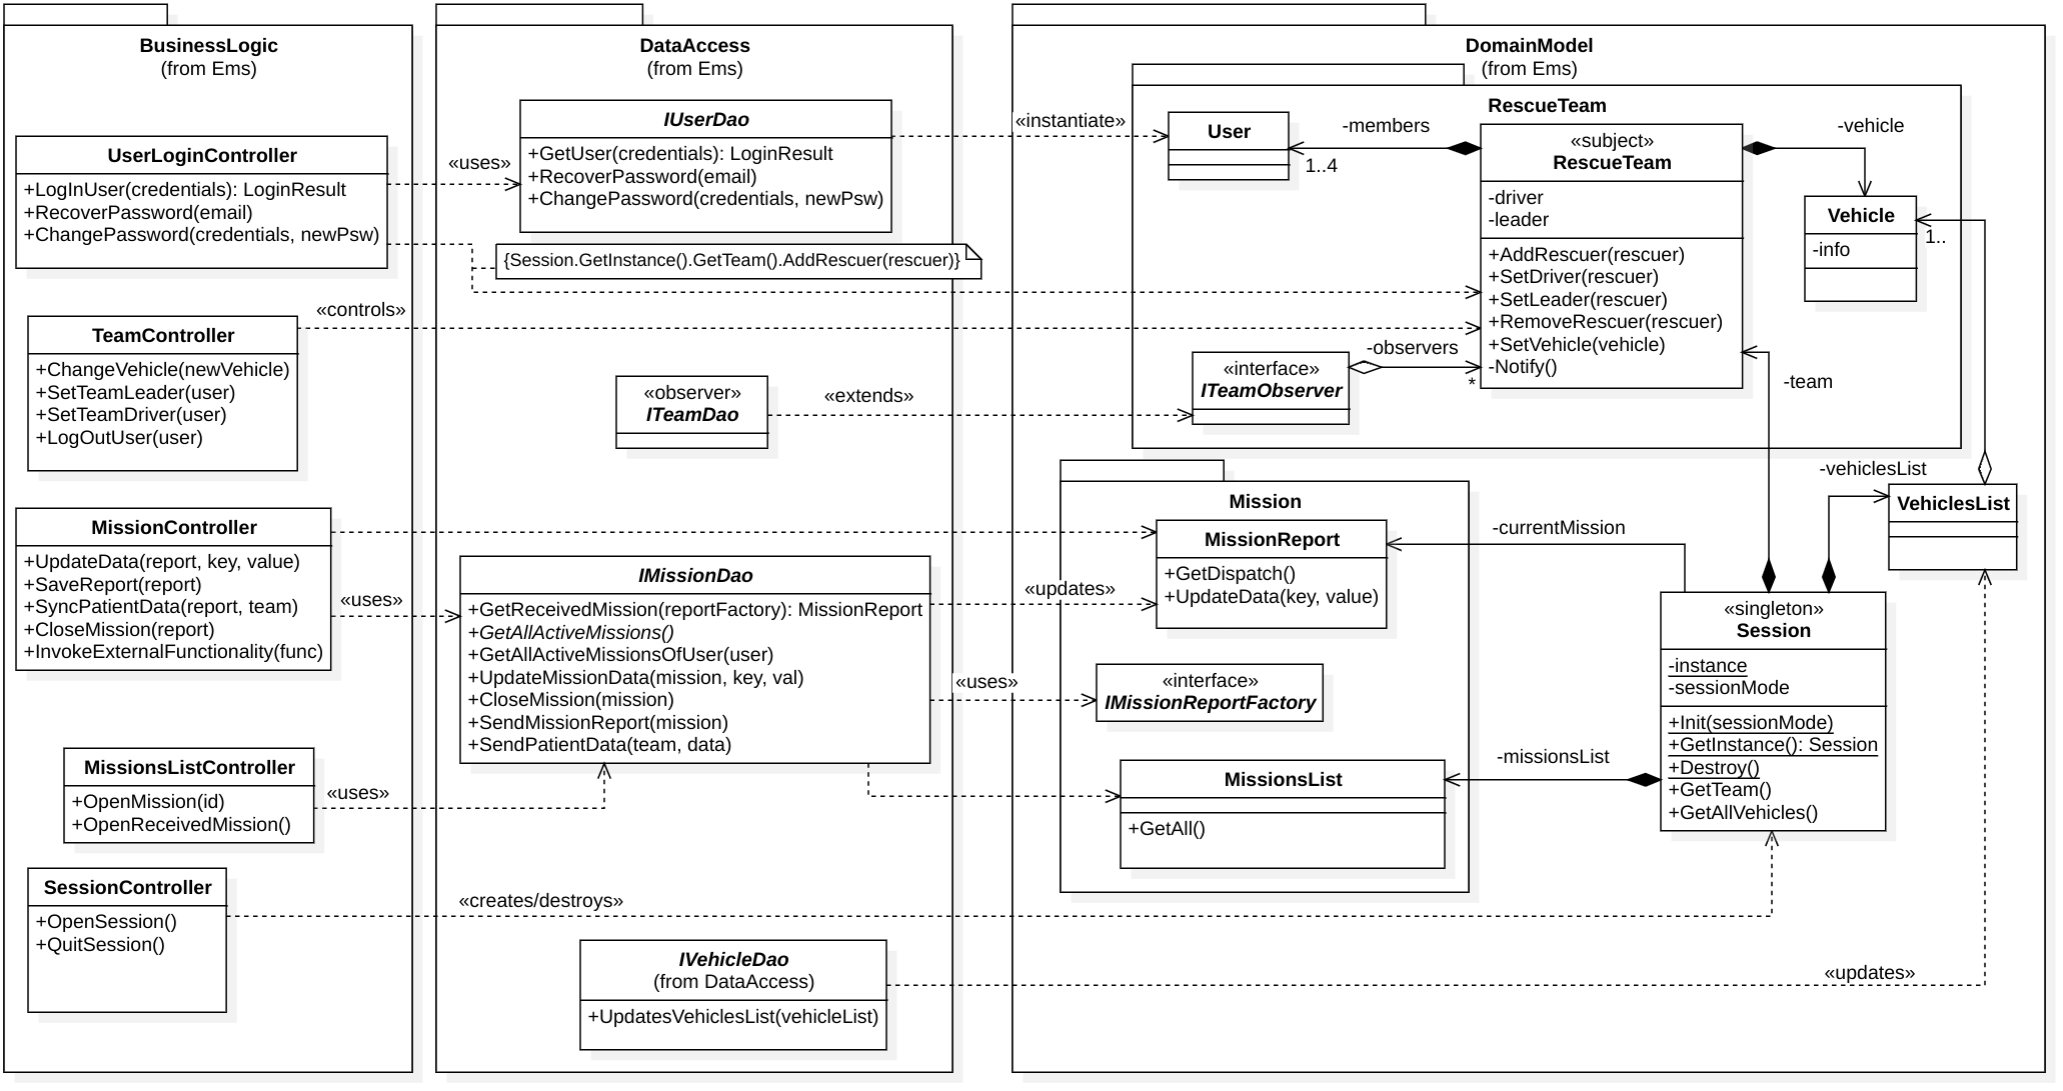
\includegraphics[width=6in]{diagrams/png/uml-ems.png}
        \caption{Diagramma delle classi di Ems}
        \label{fig:uml-ems}
    \end{figure}
    \subsubsection{Domain model di Ems}
    \begin{figure}[!h]
        \centering
        %\includesvg[width=5.4in]{diagrams/svg/Ems!EmsDomainModel_2}
        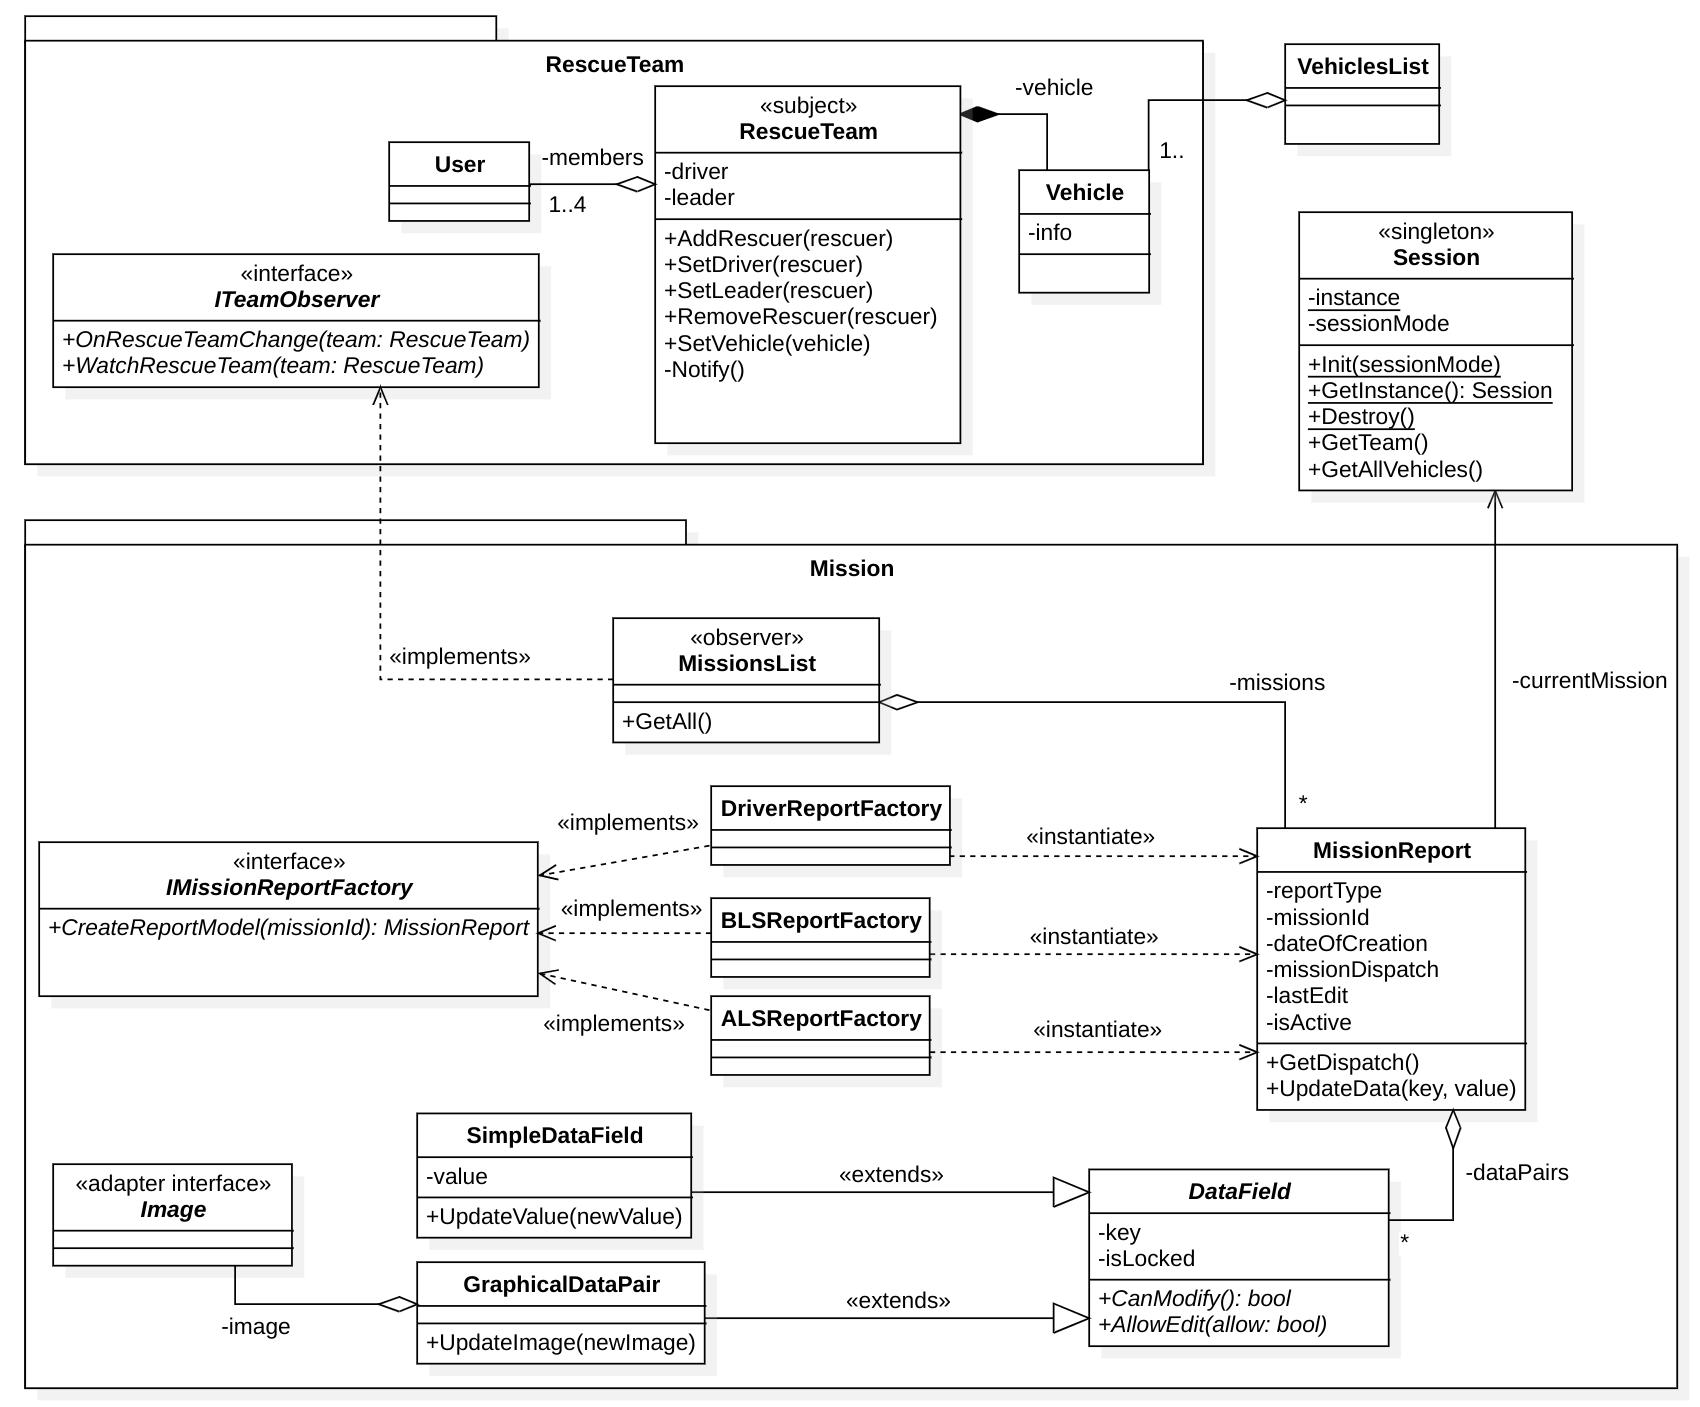
\includegraphics[width=5.4in]{diagrams/png/uml-ems-domain.png}
        \caption{Domain model del package Ems}
        \label{fig:uml-ems-domainmodel}
    \end{figure}
    Il $DomainModel$ in figura \ref{fig:uml-ems-domainmodel} contiene le classi $Session$ e $VehiclesList$ ed è suddiviso nei package $RescueTeam$ e $Mission$.
    $VehiclesList$ è una lista di $Vehicle$. $Session$ è un $Singleton$ che tiene un riferimento alla squadra corrente e alla missione in corso.
    A seconda della modalità del dispositivo (ALS, BLSD, o Autista), la $Session$ va inizializzata di conseguenza.
    $RescueTeam$ contiene l'omonima classe e le classi accessorie che caratterizzano una squadra di soccorso, ovvero $User$ e $Vehicle$.
    La classe $RescueTeam$ costituisce il $Subject$ del design pattern $Observer$, poiché quando viene modifica è necessario notificare la centrale di controllo tramite un oggetto che implementa $ITeamDao$.
    \newline Il package $Mission$ contiene $MissionReport$ e le classi responsabili della sua creazione e gestione.
    \newline Come è stato detto precedentemente, il tipo di $MissionReport$ da inizializzare è legato alla modalità con cui è stata avviata la $Session$.
    Quindi nel suo costruttore viene istanziata la giusta $Factory$ che si occupa di creare un report e aggiungerci i giusti $DataField$, che sono i possibili campi che la squadra può compilare.
    Per esempio, una squadra $BLSD$ non può avere sulla scheda il campo relativo alla somministrazione farmaci, oppure l'autista non può scrivere sulla sua scheda i parametri vitali del paziente.
    I $DataField$ possono essere campi semplici di tipo $SimpleDataField$ o contenere un elemento grafico, cioè dei $GraphicalDataPair$.
    Quest'ultimi contengono un riferimento a un'interfaccia $Adapter$ per poter gestire gli elementi grafici delle varie librerie/framework per le $GUI$.
    La classe $DataField$ è astratta e liberamente estendibile.

    \subsubsection{Organization}
    Qui, in figura \ref{fig:uml-organization}, la $BusinessLogic$ è composta da cinque $controller$: $VehicleRegistrationController$, $VehicleController$, $UserController$, $UserRegistrationController$ e $ReportsController$.
    Ognuno di questi offre operazioni $CRUD$ sulle banche dati dei veicoli, utenti e report di missione, accedendovi tramite le interfacce $IVehicleDao$, $IUserDao$ e $IReportDao$.
    Similmente al package $ControlCenter$, il modello di dominio è principalmente costituito da delle classi $Wrapper$ di liste di oggetti $Vehicle$ e $User$, che sono $VehiclesRegistry$ e $UsersRegistry$.
    In particolare, $User$ è una classe $Proxy$ in quanto un utente ha le certificazioni (di guida in emergenza, soccorso avanzato o superiori) che potrebbero essere oggetti pesanti e quindi sarebbe preferibile poterle scaricare in un secondo momento e solo se necessarie.
    \newline Per gli oggetti $Report$ invece si è ritenuto più opportuno non creare un $ReportRegistry$ poiché sui report di missione non si possono svolgere delle vere e proprie operazioni $CRUD$, se non quella di download.
    Piuttosto si è preferito implementare nella lato $BusinessLogic$ un metodo di ricerca dei report che, dato un filtro (un oggetto che implementa l'interfaccia $SearchFilter$ per formare un pattern $Strategy$) e un parametro di ricerca, restituisce una lista di risultati.
    Questo pattern è stato applicato anche in $UserController$.
    \begin{figure}[!h]
        \centering
        %\includesvg[width=6in]{diagrams/svg/Organization!Organization_3}
        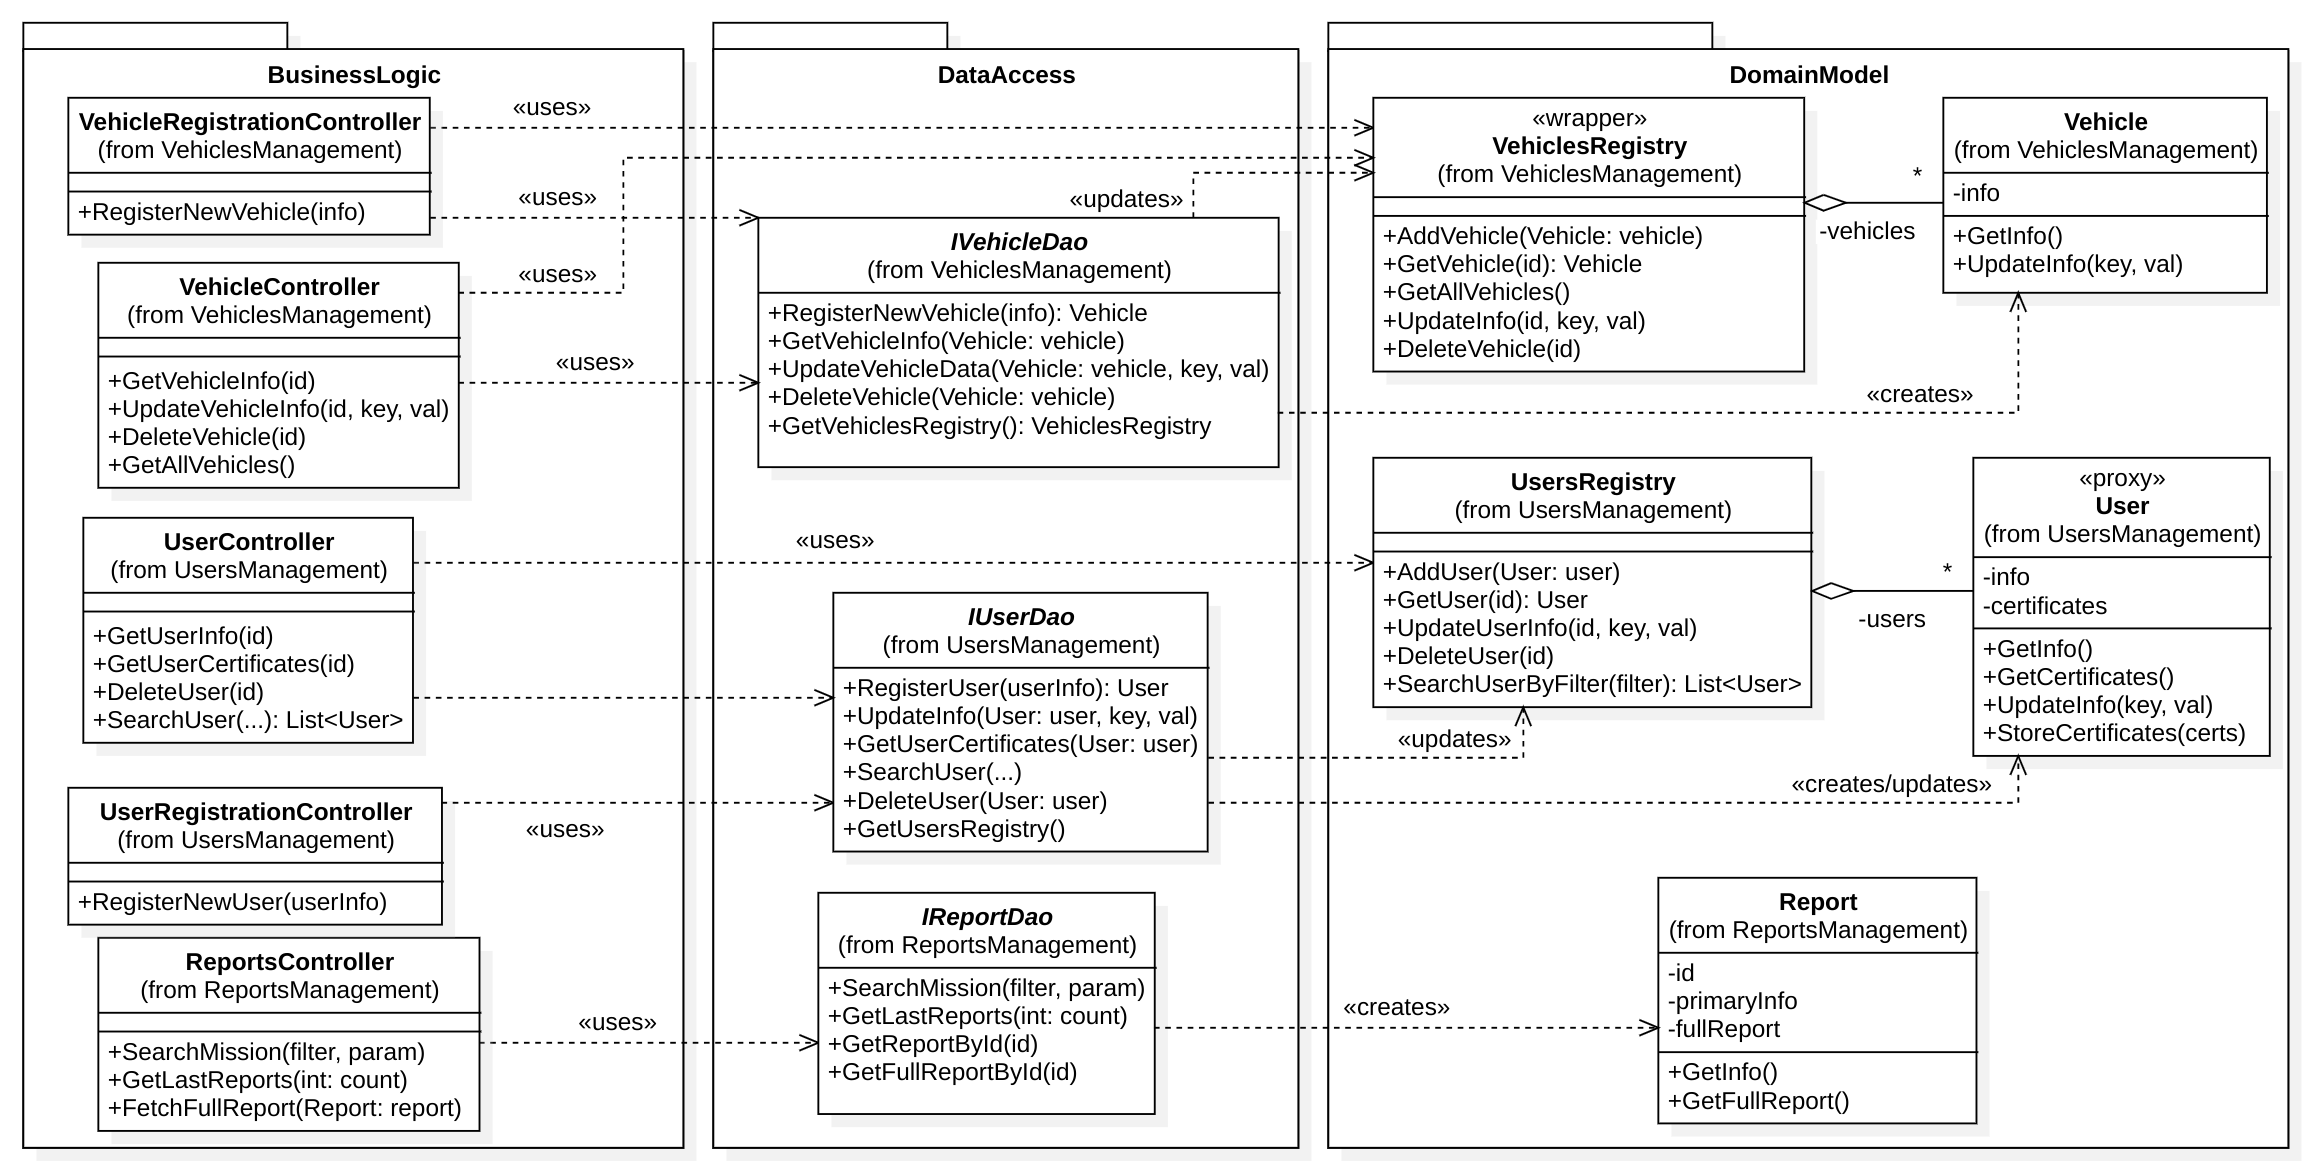
\includegraphics[width=6in]{diagrams/png/uml-organization.png}
        \caption{Diagramma delle classi di Organization}
        \label{fig:uml-organization}
    \end{figure}

    \newpage
    \subsection{Testing}
    I target principali dei test sono tutte le classi che compongono la $BusinessLogic$ di tutto l'ecosistema.
    I test formulati hanno l'obiettivo di verificare che ogni sottosistema risponda correttamente all'utente nelle situazioni normali e che fallisca correttamente nelle situazioni
    anomale identificate negli "Alternative flow" e "Non-functional requirements" dei templates dei casi d'uso.
    I test sono stati implementati con JUnit 4.

    \section{Appendice}
    \subsection{Use-case templates}
    Di seguito vengono mostrati gli use-case templates descritti con la seguente struttura:
    \begin{itemize}
        \item History:
        \item Source:
        \item Abstraction level:
        \item Description:
        \item Scope:
        \item Actors:
        \item Pre-conditions:
        \item Post-conditions:
        \item Normal flow:
        \item Variations:
        \item Alternative flow:
        \item Non-functional requirements:
    \end{itemize}
    \def\graycolor{gray!15}
    \def\creationDate{Creato il 19/02/24.\space}
    \begin{table}[!h]
        \rowcolors{2}{\graycolor}{white}
        \begin{tabularx}{\textwidth}{l|X}
            Use case & \textbf{1.1 – Riceve informazioni del chiamante} \\
            \hline
            History & \creationDate \\
            Source & Estratto dallo statement iniziale \\
            Abstraction level & User-goal \\
            Description & La centrale riceve informazioni del chiamante e la posizione della chiamata se questa viene fatta con l’ausilio dell’app di geo-localizzazione. Vedi punto A in figura \ref{fig:mockup-controlcenter}.\\
            Scope & Applicativo telematico della sala di controllo \\
            Actors & Centrale \\
            Pre-conditions & \dots \\
            Post-conditions & Deve essere salvato l’orario di ricezione della chiamata. \\
            Normal flow & \dots \\
            Variations & \dots \\
            Alternative flow & \dots \\
            Non-functional requirements & \dots
        \end{tabularx}
        \label{tab:usecase1.1}
    \end{table}

    \begin{table}[!h]
        \rowcolors{2}{\graycolor}{white}
        \begin{tabularx}{\textwidth}{l|X}
            Use case & \textbf{1.2 - Inizia nuova missione}\\
            \hline
            History & \creationDate \\
            Source & Estratto dallo statement iniziale\\
            Abstraction level & User-goal\\
            Description & La centrale crea una nuova missione tramite l’interfaccia. Vedi punto B in figura \ref{fig:mockup-controlcenter}.\\
            Scope & Applicativo telematico della sala di controllo \\
            Actors & Centrale\\
            Pre-conditions & \dots \\
            Post-conditions & Deve essere salvato l’orario di creazione della missione.\\
            Normal flow & \dots \\
            Variations & \dots \\
            Alternative flow & \dots \\
            Non-functional requirements & \dots
        \end{tabularx}
        \label{tab:usecase1.2}
    \end{table}

    \begin{table}
        \rowcolors{2}{\graycolor}{white}
        \begin{tabularx}{\textwidth}{l|X}
            Use case & \textbf{1.3 - Inserisci informazioni reperite} \\
            \hline
            History & \creationDate \\
            Source & Estratto dallo statement iniziale \\
            Abstraction level & User-goal \\
            Description & La centrale scrive il dispatch e le informazioni fornite dal chiamante che vengono successivamente allegate alla missione. Vedi punto C in figura \ref{fig:mockup-controlcenter}.\\
            Scope & Applicativo telematico della sala di controllo \\
            Actors & Centrale \\
            Pre-conditions & La missione deve essere creata. \\
            Post-conditions & \dots \\
            Normal flow & \dots \\
            Variations & \dots \\
            Alternative flow & \dots \\
            Non-functional requirements & \dots
        \end{tabularx}
        \label{tab:usecase1.3}
    \end{table}

    \begin{table}
        \rowcolors{2}{\graycolor}{white}
        \begin{tabularx}{\textwidth}{l|X}
            Use case & \textbf{1.4 - Assegna missione e invia scheda} \\
            \hline
            History & \creationDate Ultima modifica il 06/03/24.\\
            Source & Estratto dallo statement iniziale \\
            Abstraction level & User-goal \\
            Description & La centrale assegna la missione appena creata a una o più squadre di soccorso. Vedi punto D in figura \ref{fig:mockup-controlcenter}.\\
            Scope & Applicativo telematico della sala di controllo \\
            Actors & Centrale, squadre di soccorso \\
            Pre-conditions & La missione deve essere creata. La squadra non deve essere impegnata in un'altra missione.\\
            Post-conditions & Ciascuna squadra ottiene una scheda relativa alla missione \\
            Normal flow & \dots \\
            Variations & \dots \\
            Alternative flow & \dots \\
            Non-functional requirements & \dots
        \end{tabularx}
        \label{tab:usecase1.4}
    \end{table}

    \begin{table}
        \rowcolors{2}{\graycolor}{white}
        \begin{tabularx}{\textwidth}{l|X}
            Use case & \textbf{1.5 - Specifica codice di attivazione} \\
            \hline
            History & \creationDate Ultima modifica il 06/03/24.\\
            Source & Estratto dallo statement iniziale \\
            Abstraction level & User-goal \\
            Description & La centrale specifica il codice di attivazione della missione. Vedi punto E in figura \ref{fig:mockup-controlcenter}.\\
            Scope & Applicativo telematico della sala di controllo\\
            Actors & Centrale, squadre di soccorso \\
            Pre-conditions & La missione deve essere creata. La squadra non deve essere impegnata in un'altra missione.\\
            Post-conditions & Ciascuna squadra ottiene la scheda con il codice di attivazione della missione. \\
            Normal flow & \dots \\
            Variations & \dots \\
            Alternative flow & \dots \\
            Non-functional requirements & \dots
        \end{tabularx}
        \label{tab:usecase1.5}
    \end{table}

    \begin{table}
        \rowcolors{2}{\graycolor}{white}
        \begin{tabularx}{\textwidth}{l|X}
            Use case & \textbf{1.6 - Aggiorna dispatch} \\
            \hline
            History & \creationDate \\
            Source & Proposto per migliorare l'interazione tra centrale e squadre di soccorso. \\
            Abstraction level & User-goal \\
            Description & La centrale aggiorna le informazioni nel dispatch della missione. Vedi punto F in figura \ref{fig:mockup-controlcenter}.\\
            Scope & Applicativo telematico della sala di controllo\\
            Actors & Centrale, squadre di soccorso \\
            Pre-conditions & La missione deve essere creata. \\
            Post-conditions & Ciascuna squadra riceve le modifiche effettuate al dispatch nella scheda della missione. \\
            Normal flow & \dots \\
            Variations & \dots \\
            Alternative flow & \dots \\
            Non-functional requirements & \dots
        \end{tabularx}
        \label{tab:usecase1.6}
    \end{table}

    \begin{table}
        \rowcolors{2}{\graycolor}{white}
        \begin{tabularx}{\textwidth}{l|X}
            Use case & \textbf{1.7 - Osserva posizioni mezzi} \\
            \hline
            History & \creationDate \\
            Source & Estratto dallo statement iniziale \\
            Abstraction level & User-goal \\
            Description & La centrale può osservare la posizione attuale di ogni squadra. Vedi mappa in figura \ref{fig:mockup-controlcenter}.\\
            Scope & Applicativo telematico della sala di controllo\\
            Actors & Centrale, squadre di soccorso \\
            Pre-conditions & \dots \\
            Post-conditions & \dots \\
            Normal flow & \dots \\
            Variations & \dots \\
            Alternative flow & \dots \\
            Non-functional requirements & \dots
        \end{tabularx}
        \label{tab:usecase1.7}
    \end{table}

    \begin{table}
        \rowcolors{2}{\graycolor}{white}
        \begin{tabularx}{\textwidth}{l|X}
            Use case & \textbf{2.1 – Riceve scheda missione}\\
            \hline
            History & \creationDate \\
            Source & Estratto dallo statement iniziale\\
            Abstraction level & User-goal\\
            Description & La squadra riceve la scheda missione\\
            Scope & Applicativo telematico della squadra di soccorso\\
            Actors & Squadra\\
            Pre-conditions & \dots \\
            Post-conditions & \dots \\
            Normal flow & \dots \\
            Variations & \dots \\
            Alternative flow & \dots \\
            Non-functional requirements & \dots
        \end{tabularx}
        \label{tab:usecase2.1}
    \end{table}

    \begin{table}
        \rowcolors{2}{\graycolor}{white}
        \begin{tabularx}{\textwidth}{l|X}
            Use case & \textbf{2.2 – Apre scheda missione}\\
            \hline
            History & \creationDate \\
            Source & Estratto dallo statement iniziale\\
            Abstraction level & Function\\
            Description & La squadra apre la scheda missione per iniziare la compilazione dei dati/parametri.\\
            Scope & Applicativo telematico della squadra di soccorso\\
            Actors & Squadra\\
            Pre-conditions & \dots \\
            Post-conditions & \dots \\
            Normal flow & \dots \\
            Variations & \dots \\
            Alternative flow & \dots \\
            Non-functional requirements & \dots
        \end{tabularx}
        \label{tab:usecase2.2}
    \end{table}

    \begin{table}
        \rowcolors{2}{\graycolor}{white}
        \begin{tabularx}{\textwidth}{l|X}
            Use case & \textbf{2.3 – Inserisci dati anagrafici}\\
            \hline
            History & \creationDate Ultima modifica il 06/03/24.\\
            Source & Estratto dallo statement iniziale\\
            Abstraction level & User-goal\\
            Description & Il soccorritore annota i dati anagrafici del paziente. Vedi punto A in figura \ref{fig:mockup-soccorritore}.\\
            Scope & Applicativo telematico della squadra di soccorso\\
            Actors & Squadra\\
            Pre-conditions & \dots \\
            Post-conditions & \dots \\
            Normal flow & \dots \\
            Variations & Vedi 2.2 \\
            Alternative flow & \dots \\
            Non-functional requirements & Se la connessione è presente, i dati vengono inviati automaticamente alla centrale.
        \end{tabularx}
        \label{tab:usecase2.3}
    \end{table}

    \begin{table}
        \rowcolors{2}{\graycolor}{white}
        \begin{tabularx}{\textwidth}{l|X}
            Use case & \textbf{2.4 – Calcola dati anagrafici da codice fiscale}\\
            \hline
            History & \creationDate Ultima modifica il 06/03/24.\\
            Source & Estratto dallo statement iniziale\\
            Abstraction level & Function \\
            Description & Il soccorritore compila i dati anagrafici del paziente automaticamente inserendo solamente il codice fiscale. Vedi punto B in figura \ref{fig:mockup-soccorritore}.\\
            Scope & Applicativo telematico della squadra di soccorso\\
            Actors & Squadra\\
            Pre-conditions & \dots \\
            Post-conditions & \dots \\
            Normal flow & \dots \\
            Variations & \dots \\
            Alternative flow & \dots \\
            Non-functional requirements & Se la connessione è presente, i dati vengono inviati automaticamente alla centrale.
        \end{tabularx}
        \label{tab:usecase2.4}
    \end{table}

    \begin{table}
        \rowcolors{2}{\graycolor}{white}
        \begin{tabularx}{\textwidth}{l|X}
            Use case & \textbf{2.5 – Inserisci parametri vitali}\\
            \hline
            History & \creationDate Ultima modifica il 06/03/24.\\
            Source & Estratto dallo statement iniziale\\
            Abstraction level & User-goal\\
            Description & Il soccorritore inserisce i parametri vitali del paziente. Vedi punto C in figura \ref{fig:mockup-soccorritore}.\\
            Scope & Applicativo telematico della squadra di soccorso\\
            Actors & Squadra\\
            Pre-conditions & \dots \\
            Post-conditions & \dots \\
            Normal flow & \dots \\
            Variations & \dots \\
            Alternative flow & \dots \\
            Non-functional requirements & Se la connessione è presente, i dati vengono inviati automaticamente alla centrale.
        \end{tabularx}
        \label{tab:usecase2.5}
    \end{table}

    \begin{table}
        \rowcolors{2}{\graycolor}{white}
        \begin{tabularx}{\textwidth}{l|X}
            Use case & \textbf{2.6 – Inserisci firma del paziente}\\
            \hline
            History & \creationDate Ultima modifica il 06/03/24.\\
            Source & Estratto dallo statement iniziale\\
            Abstraction level & User-goal\\
            Description & Il soccorritore fa firmare il rifiuto di trasporto al paziente. Vedi punto D in figura \ref{fig:mockup-soccorritore}.\\
            Scope & Applicativo telematico della squadra di soccorso\\
            Actors & Squadra\\
            Pre-conditions & Esito trattamento “rifiuto trasporto”. \\
            Post-conditions & \dots \\
            Normal flow & \dots \\
            Variations & \dots \\
            Alternative flow & \dots \\
            Non-functional requirements & Se la connessione è presente, la firma viene inviata automaticamente alla centrale.
        \end{tabularx}
        \label{tab:usecase2.6}
    \end{table}

    \begin{table}
        \rowcolors{2}{\graycolor}{white}
        \begin{tabularx}{\textwidth}{l|X}
            Use case & \textbf{2.7 – Sincronizza dati e parametri con la centrale}\\
            \hline
            History & \creationDate \\
            Source & Estratto dallo statement iniziale\\
            Abstraction level & User-goal\\
            Description & Il soccorritore sincronizza manualmente i dati e i parametri vitali con la centrale. Vedi punto E in figura \ref{fig:mockup-soccorritore}.\\
            Scope & Applicativo telematico della squadra di soccorso\\
            Actors & Squadra\\
            Pre-conditions & \dots \\
            Post-conditions & \dots \\
            Normal flow & \dots \\
            Variations & \dots \\
            Alternative flow & \dots \\
            Non-functional requirements & \dots
        \end{tabularx}
        \label{tab:usecase2.7}
    \end{table}

    \begin{table}
        \rowcolors{2}{\graycolor}{white}
        \begin{tabularx}{\textwidth}{l|X}
            Use case & \textbf{2.8 – Condividi dati con altre squadre}\\
            \hline
            History & \creationDate Ultima modifica il 08/03/24\\
            Source & Estratto dallo statement iniziale\\
            Abstraction level & User-goal\\
            Description & Il soccorritore condivide i dati anagrafici con altre squadre giunte in supporto. Vedi punto F in figura \ref{fig:mockup-soccorritore}.\\
            Scope & Applicativo telematico della squadra di soccorso\\
            Actors & Squadra\\
            Pre-conditions & La squadra ricevente deve essere assegnata alla stessa missione \\
            Post-conditions & \dots \\
            Normal flow & a. Inserire numero della squadra ricevente\newline b. La squadra ricevente accetta o rifiuta i dati ricevuti.\\
            Variations & \dots \\
            Alternative flow & \dots \\
            Non-functional requirements & \dots
        \end{tabularx}
        \label{tab:usecase2.8}
    \end{table}

    \begin{table}
        \rowcolors{2}{\graycolor}{white}
        \begin{tabularx}{\textwidth}{l|X}
            Use case & \textbf{2.9 – Firma la scheda}\\
            \hline
            History & \creationDate \\
            Source & Estratto dallo statement iniziale\\
            Abstraction level & Function\\
            Description & La squadra firma e chiude la scheda della missione. Vedi punto G in figura \ref{fig:mockup-soccorritore}.\\
            Scope & Applicativo telematico della squadra di soccorso\\
            Actors & Squadra\\
            Pre-conditions & Tutti i campi devono essere compilati \\
            Post-conditions & La scheda rimane immutabile \\
            Normal flow & \dots \\
            Variations & \dots \\
            Alternative flow & \dots \\
            Non-functional requirements & \dots
        \end{tabularx}
        \label{tab:usecase2.9}
    \end{table}

    \begin{table}
        \rowcolors{2}{\graycolor}{white}
        \begin{tabularx}{\textwidth}{l|X}
            Use case & \textbf{2.10 – Seleziona mezzo}\\
            \hline
            History & \creationDate \\
            Source & Estratto dallo statement iniziale\\
            Abstraction level & Function\\
            Description & La squadra cambia il mezzo di soccorso selezionandone uno diverso tra quelli disponibili\\
            Scope & Applicativo telematico della squadra di soccorso\\
            Actors & Squadra\\
            Pre-conditions & \dots \\
            Post-conditions & \dots \\
            Normal flow & \dots \\
            Variations & \dots \\
            Alternative flow & \dots \\
            Non-functional requirements & \dots
        \end{tabularx}
        \label{tab:usecase2.10}
    \end{table}

    \begin{table}
        \rowcolors{2}{\graycolor}{white}
        \begin{tabularx}{\textwidth}{l|X}
            Use case & \textbf{2.11 – Seleziona caposquadra}\\
            \hline
            History & \creationDate \\
            Source & Estratto dallo statement iniziale\\
            Abstraction level & Function\\
            Description & La squadra cambia il caposquadra selezionando uno dei soccorritori loggati.\\
            Scope & Applicativo telematico della squadra di soccorso\\
            Actors & Squadra\\
            Pre-conditions & Almeno un soccorritore loggato. \\
            Post-conditions & \dots \\
            Normal flow & \dots \\
            Variations & \dots \\
            Alternative flow & \dots \\
            Non-functional requirements & \dots
        \end{tabularx}
        \label{tab:usecase2.11}
    \end{table}

    \begin{table}
        \rowcolors{2}{\graycolor}{white}
        \begin{tabularx}{\textwidth}{l|X}
            Use case & \textbf{2.12 – Seleziona autista}\\
            \hline
            History & \creationDate \\
            Source & Estratto dallo statement iniziale\\
            Abstraction level & Function\\
            Description & La squadra cambia l’autista selezionando uno dei soccorritori loggati.\\
            Scope & Applicativo telematico della squadra di soccorso\\
            Actors & Squadra\\
            Pre-conditions & Almeno un soccorritore loggato. \\
            Post-conditions & \dots \\
            Normal flow & \dots \\
            Variations & \dots \\
            Alternative flow & \dots \\
            Non-functional requirements & \dots
        \end{tabularx}
        \label{tab:usecase2.12}
    \end{table}

    \begin{table}
        \rowcolors{2}{\graycolor}{white}
        \begin{tabularx}{\textwidth}{l|X}
            Use case & \textbf{2.13 – Login}\\
            \hline
            History & \creationDate \\
            Source & Estratto dallo statement iniziale\\
            Abstraction level & Function\\
            Description & Il soccorritore effettua il login inserendo le proprie credenziali.\\
            Scope & Applicativo telematico della squadra di soccorso\\
            Actors & Soccorritore\\
            Pre-conditions & Il soccorritore deve essere registrato presso l’associazione. \\
            Post-conditions & \dots \\
            Normal flow & a. Inserisce nome utente e password\newline b. Login effettuato \\
            Variations & \dots\\
            Alternative flow & a1. Password errata. Ritorna al punto (a) \newline a2. Password scaduta. Cambia password: vedi 2.15  \\
            Non-functional requirements & Viene aggiornata la lista delle missioni aperte, mostrando solamente
            quelle che coinvolgono i membri della squadra.
        \end{tabularx}
        \label{tab:usecase2.13}
    \end{table}

    \begin{table}
        \rowcolors{2}{\graycolor}{white}
        \begin{tabularx}{\textwidth}{l|X}
            Use case & \textbf{2.14 – Recupera password}\\
            \hline
            History & \creationDate \\
            Source & Estratto dallo statement iniziale\\
            Abstraction level & Function\\
            Description & Il soccorritore recupera la password ricevendo via email il link per il reset della password.\\
            Scope & Applicativo telematico della squadra di soccorso\\
            Actors & Soccorritore\\
            Pre-conditions & Il soccorritore deve essere registrato presso l’associazione. \\
            Post-conditions & \dots \\
            Normal flow & \dots \\
            Variations & \dots \\
            Alternative flow & \dots \\
            Non-functional requirements & \dots
        \end{tabularx}
        \label{tab:usecase2.14}
    \end{table}

    \begin{table}
        \rowcolors{2}{\graycolor}{white}
        \begin{tabularx}{\textwidth}{l|X}
            Use case & \textbf{2.15 – Primo login}\\
            \hline
            History & \creationDate \\
            Source & Estratto dallo statement iniziale\\
            Abstraction level & Function\\
            Description & Il soccorritore effettua il primo login con le credenziali provvisorie.\\
            Scope & Applicativo telematico della squadra di soccorso\\
            Actors & Soccorritore\\
            Pre-conditions & Il soccorritore deve essere registrato presso l’associazione. \\
            Post-conditions & \dots \\
            Normal flow & a. Inserisce nome utente e password provvisoria\newline b. Cambia password: vedi 2.15.\newline c. Effettua login con la nuova password: vedi 2.12 \\
            Variations & \dots \\
            Alternative flow & \dots \\
            Non-functional requirements & \dots
        \end{tabularx}
        \label{tab:usecase2.15}
    \end{table}

    \begin{table}
        \rowcolors{2}{\graycolor}{white}
        \begin{tabularx}{\textwidth}{l|X}
            Use case & \textbf{2.16 – Cambia password}\\
            \hline
            History & \creationDate \\
            Source & Estratto dallo statement iniziale\\
            Abstraction level & Function\\
            Description & Il soccorritore cambia password inserendo quella vecchia e quella nuova.\\
            Scope & Applicativo telematico della squadra di soccorso\\
            Actors & Soccorritore\\
            Pre-conditions & Il soccorritore deve essere registrato presso l’associazione. \\
            Post-conditions & Il soccorritore ha una nuova password \\
            Normal flow & \dots \\
            Variations & \dots \\
            Alternative flow & \dots \\
            Non-functional requirements & \dots
        \end{tabularx}
        \label{tab:usecase2.16}
    \end{table}

    \begin{table}
        \rowcolors{2}{\graycolor}{white}
        \begin{tabularx}{\textwidth}{l|X}
            Use case & \textbf{2.17 – Logout}\\
            \hline
            History & \creationDate Ultima modifica il 21/02/24 \\
            Source & Estratto dallo statement iniziale\\
            Abstraction level & Function\\
            Description & Il soccorritore effettua il logout\\
            Actors & Soccorritore\\
            Pre-conditions & Il soccorritore deve essere registrato e loggato nella sessione. \\
            Post-conditions & Il soccorritore viene sloggato dalla sessione. \\
            Normal flow & \dots \\
            Variations & \dots \\
            Alternative flow & \dots \\
            Non-functional requirements & Viene aggiornata la lista delle missioni aperte, mostrando solamente quelle che coinvolgono i membri della squadra.
        \end{tabularx}
        \label{tab:usecase2.17}
    \end{table}

    \begin{table}
        \rowcolors{2}{\graycolor}{white}
        \begin{tabularx}{\textwidth}{l|X}
            Use case & \textbf{3.1 – Apre scheda-missione}\\
            \hline
            History & Creato il 22/02/24\\
            Source & Estratto dallo statement iniziale\\
            Abstraction level & User-goal\\
            Description & L'autista riceve e apre la scheda missione appena ricevuta per iniziare la compilazione e invio stati.\\
            Scope & Applicativo telematico dell'autista della squadra di soccorso\\
            Actors & Autista\\
            Pre-conditions & \dots \\
            Post-conditions & \dots \\
            Normal flow & \dots\\
            Variations & Vedi 3.2 \\
            Alternative flow & \dots \\
            Non-functional requirements & \dots
        \end{tabularx}
        \label{tab:usecase3.1}
    \end{table}

    \begin{table}
        \rowcolors{2}{\graycolor}{white}
        \begin{tabularx}{\textwidth}{l|X}
            Use case & \textbf{3.2 – Passa a nuova missione appena ricevuta}\\
            \hline
            History & Creato il 22/02/24\\
            Source & Estratto dallo statement iniziale\\
            Abstraction level & Function\\
            Description & L'autista apre la scheda missione appena ricevuta per iniziare la compilazione e invio stati.\\
            Scope & Applicativo telematico dell'autista della squadra di soccorso\\
            Actors & Autista\\
            Pre-conditions & Stato di "rientro in sede" ancora non inviato \\
            Post-conditions & \dots \\
            Normal flow & a. Inserire il chilometraggio attuale del veicolo\newline b. Aprire scheda-missione (4.1)\\
            Variations & \dots \\
            Alternative flow & \dots \\
            Non-functional requirements & \dots
        \end{tabularx}
        \label{tab:usecase3.2}
    \end{table}

    \begin{table}
        \rowcolors{2}{\graycolor}{white}
        \begin{tabularx}{\textwidth}{l|X}
            Use case & \textbf{3.3 – Invia stato missione}\\
            \hline
            History & Creato il 22/02/24\\
            Source & Estratto dallo statement iniziale\\
            Abstraction level & User-goal\\
            Description & L'autista invia lo stato di missione ogni qualvolta il mezzo si muova. Vedi punto A in figura \ref{fig:mockup-autista}.\\
            Scope & Applicativo telematico dell'autista della squadra di soccorso\\
            Actors & Autista\\
            Pre-conditions & \dots \\
            Post-conditions & Viene salvato l'orario di invio dello stato. \\
            Normal flow & \dots\\
            Variations & \dots \\
            Alternative flow & \dots \\
            Non-functional requirements & \dots
        \end{tabularx}
        \label{tab:usecase3.3}
    \end{table}

    \begin{table}
        \rowcolors{2}{\graycolor}{white}
        \begin{tabularx}{\textwidth}{l|X}
            Use case & \textbf{3.4 – Salva orario}\\
            \hline
            History & Creato il 22/02/24\\
            Source & Proposto per gestire il caso in cui l'autista si possa dimenticare di inviare lo stato, o lo faccia troppo tardi.\\
            Abstraction level & User-goal \\
            Description & Salva o modifica l'orario di invio di uno stato. Vedi punto B in figura \ref{fig:mockup-autista}.\\
            Scope & Applicativo telematico dell'autista della squadra di soccorso\\
            Actors & Autista\\
            Pre-conditions & Per modificare l'orario di uno stato è necessario aver inviato tale stato.\\
            Post-conditions & \dots \\
            Normal flow & \dots\\
            Variations & \dots \\
            Alternative flow & \dots \\
            Non-functional requirements & \dots
        \end{tabularx}
        \label{tab:usecase3.4}
    \end{table}

    \begin{table}
        \rowcolors{2}{\graycolor}{white}
        \begin{tabularx}{\textwidth}{l|X}
            Use case & \textbf{3.5 – Invia esito della missione}\\
            \hline
            History & Creato il 22/02/24\\
            Source & Estratto dallo statement iniziale\\
            Abstraction level & User-goal\\
            Description & Invia l'esito della missione quando la squadra sta per abbandonare l'obiettivo. Vedi punto C in figura \ref{fig:mockup-autista}.\\
            Scope & Applicativo telematico dell'autista della squadra di soccorso\\
            Actors & Autista\\
            Pre-conditions & Stato "arrivo su obiettivo" raggiunto. \\
            Post-conditions & \dots \\
            Normal flow & \dots\\
            Variations & \dots \\
            Alternative flow & \dots \\
            Non-functional requirements & \dots
        \end{tabularx}
        \label{tab:usecase3.5}
    \end{table}

    \begin{table}
        \rowcolors{2}{\graycolor}{white}
        \begin{tabularx}{\textwidth}{l|X}
            Use case & \textbf{3.6 – Imposta navigatore}\\
            \hline
            History & Creato il 22/02/24\\
            Source & Estratto dallo statement iniziale\\
            Abstraction level & User-goal\\
            Description & Imposta navigatore per raggiungere l'obiettivo o la destinazione\\
            Scope & Applicativo telematico dell'autista della squadra di soccorso\\
            Actors & Autista\\
            Pre-conditions & \dots \\
            Post-conditions & \dots \\
            Normal flow & \dots\\
            Variations & \dots \\
            Alternative flow & \dots \\
            Non-functional requirements & \dots
        \end{tabularx}
        \label{tab:usecase3.6}
    \end{table}

    \begin{table}
        \rowcolors{2}{\graycolor}{white}
        \begin{tabularx}{\textwidth}{l|X}
            Use case & \textbf{3.7 – Inserisci chilometraggio del mezzo}\\
            \hline
            History & Creato il 22/02/24\\
            Source & Estratto dallo statement iniziale\\
            Abstraction level & Function\\
            Description & Inserisce chilometraggio del mezzo. Vedi punto D in figura \ref{fig:mockup-autista}.\\
            Scope & Applicativo telematico dell'autista della squadra di soccorso\\
            Actors & Autista\\
            Pre-conditions & \dots \\
            Post-conditions & \dots \\
            Normal flow & \dots\\
            Variations & \dots \\
            Alternative flow & \dots \\
            Non-functional requirements & \dots
        \end{tabularx}
        \label{tab:usecase3.7}
    \end{table}
%%
    \def\organizationscope{Applicativo telematico dell'associazione}
    \begin{table}
        \rowcolors{2}{\graycolor}{white}
        \begin{tabularx}{\textwidth}{l|X}
            Use case & \textbf{4.1 - Gestisci mezzi} \\
            \hline
            History & \creationDate \\
            Source & Estratto dallo statement iniziale\\
            Abstraction level & Summary\\
            Description & Operazioni CRUD sul database dei veicoli dell’associazione \\
            Scope & \organizationscope\\
            Actors & Associazione\\
            Pre-conditions & Deve essere effettuato l'accesso\\
            Post-conditions & \dots \\
            Normal flow & \dots \\
            Variations & \dots \\
            Alternative flow & \dots \\
            Non-functional requirements & \dots
        \end{tabularx}
        \label{tab:usecase4.1}
    \end{table}

    \begin{table}
        \rowcolors{2}{\graycolor}{white}
        \begin{tabularx}{\textwidth}{l|X}
            Use case & \textbf{4.2 - Registra soccorritore} \\
            \hline
            History & \creationDate \\
            Source & Estratto dallo statement iniziale\\
            Abstraction level & User-goal\\
            Description & L’associazione registra un nuovo soccorritore con i dati anagrafici e email\\
            Scope & \organizationscope\\
            Actors & Associazione\\
            Pre-conditions & Deve essere effettuato l'accesso\\
            Post-conditions & \dots\\
            Normal flow & \dots \\
            Variations & \dots \\
            Alternative flow & \dots \\
            Non-functional requirements & \dots
        \end{tabularx}
        \label{tab:usecase4.2}
    \end{table}

    \begin{table}
        \rowcolors{2}{\graycolor}{white}
        \begin{tabularx}{\textwidth}{l|X}
            Use case & \textbf{4.3 - Inserisci certificazione} \\
            \hline
            History & \creationDate \\
            Source & Estratto dallo statement iniziale\\
            Abstraction level & User-goal\\
            Description & L’associazione inserisce le certificazioni ottenute dal soccorritore appena registrato\\
            Scope & \organizationscope\\
            Actors & Associazione\\
            Pre-conditions & Deve essere effettuato l'accesso. Il soccorritore deve essere registrato.\\
            Post-conditions & \dots\\
            Normal flow & \dots \\
            Variations & \dots \\
            Alternative flow & \dots \\
            Non-functional requirements & \dots
        \end{tabularx}
        \label{tab:usecase4.3}
    \end{table}

    \begin{table}
        \rowcolors{2}{\graycolor}{white}
        \begin{tabularx}{\textwidth}{l|X}
            Use case & \textbf{4.4 - Consulta schede-missione} \\
            \hline
            History & \creationDate \\
            Source & Estratto dallo statement iniziale\\
            Abstraction level & User-goal\\
            Description & L’associazione scarica tramite un identificativo tutto il report della missione\\
            Scope & \organizationscope\\
            Actors & Associazione\\
            Pre-conditions & Deve essere effettuato l'accesso.\\
            Post-conditions & \dots\\
            Normal flow & \dots \\
            Variations & \dots \\
            Alternative flow & \dots \\
            Non-functional requirements & \dots
        \end{tabularx}
        \label{tab:usecase4.4}
    \end{table}

    \begin{table}
        \rowcolors{2}{\graycolor}{white}
        \begin{tabularx}{\textwidth}{l|X}
            Use case & \textbf{4.5 - Reperisci certificazione} \\
            \hline
            History & Creato il 21/02/24 \\
            Source & Estratto dallo statement iniziale\\
            Abstraction level & User-goal\\
            Description & L’associazione reperisce le certificazioni di un soccorritore registrato.\\
            Scope & \organizationscope\\
            Actors & Associazione\\
            Pre-conditions & Deve essere effettuato l'accesso. Il soccorritore deve essere registrato.\\
            Post-conditions & \dots\\
            Normal flow & \dots \\
            Variations & \dots \\
            Alternative flow & \dots \\
            Non-functional requirements & \dots
        \end{tabularx}
        \label{tab:usecase4.5}
    \end{table}

\end{document}